\documentclass[a4paper]{article}
\usepackage[utf8]{inputenc}
\usepackage[left=3.5cm, right=3.5cm]{geometry}
\usepackage{amsmath}
\usepackage{graphicx}
\usepackage{fancyhdr}
\usepackage{hyperref}
\usepackage{enumerate}
\usepackage{amsfonts}
\usepackage{amssymb}
\usepackage{tikz}

\newcommand{\R}{\mathbb{R}}
\newcommand{\N}{\mathbb{N}}
\newcommand{\C}{\mathbb{C}}
\newcommand{\Q}{\mathbb{Q}}
\newcommand{\F}{\mathbb{F}}
\newcommand{\E}{\mathbb{E}}
\renewcommand{\P}{\mathbb{P}}
\newcommand{\f}[1]{\text{#1}}

\pagestyle{fancy}
\fancyhf{}
\lhead{\today}
\chead{CS 70}
\rhead{Albert Zhang}
\cfoot{\thepage}

\setcounter{secnumdepth}{0}
\setlength{\parindent}{0pt}

\title{CS 70 Notes \& Solutions}
\author{Albert Zhang}
\date{Year One \\ Fall Semester}

\begin{document}


\maketitle
\tableofcontents
\newpage

\include{Lec_0}
\section{Homework 0}
\begin{enumerate}
    \item (a) CS70 Website (click): \url{www.eecs70.org} \\
          (b) HW: 10\%, Midterm 1: 25\%, Midterm 2: 25\%, Final: 40\%
    \item (a) \boxed{\text{Yes.}} Alice and Bob cannot write up a solution together. They must each write up their solutions independently. \\
          (b) \boxed{\text{No.}} Taking notes is fine, as long as Carol isn't directly copying what Dan is saying. She did indeed write up her solution by herself, and credited Dan for his ideas. \\
          (c) \boxed{\text{No.}} Using the same approach from a website source is fine as long as Erin didn't copy any parts verbatim and she cites the website, which she did. \\
          (d) \boxed{\text{Yes.}} This is not fine as Frank copied Grace's written solution verbatim. Therefore, he was technically in possession of another student's solution, which makes him a naughty child. \\
          (e) \boxed{\text{Yes.}} This is not fine as Irene was in possession of another student's (Heidi's) solution.
    \item (a) The post number for the Note 0 thread is \href{https://piazza.com/class/jkjku77a1h451b?cid=13}{13} \\
          (b) Comment: "Could you be more specific? Which parts of the proof do you get (in your own words), and which parts are you having trouble with? You could also try going to office hours or a homework party."
    \item (a) $\forall x \exists y((P(x)\wedge Q(x, y)) \implies x \leq \sqrt{y})$ \\
          (b) $\sum\limits_{i=0}^k i = \frac{k(k+1)}{2}$
\end{enumerate}
\section{Homework 1}
 
Sundry? (that's some spicy vocab) :

I worked alone and TeX-ed my solutions as I solved the problems.

\begin{enumerate}
    %%%%%%%%%% TAUTOLOGY AND CONTRADICTIONS %%%%%%%%%
    \item\begin{enumerate}[(a)]
        % Part A
        \item \boxed{\text{Contradiction.}} \newline 
        \begin{tabular}{c|c|c|c|c}
            x & y & x$\Rightarrow$y & $\neg$y & (a) \\ \hline
            T & T & T & F & F \\ \hline
            T & F & F & T & F \\ \hline
            F & T & T & F & F \\ \hline
            F & F & T & T & F
        \end{tabular}
        % Part B
        \item \boxed{\text{Tautology.}} \newline
        \begin{tabular}{c|c|c|c}
            x & y & x$\vee$y & (b) \\ \hline
            T & T & T & T \\ \hline
            T & F & T & T \\ \hline
            F & T & T & T \\ \hline
            F & F & F & T
        \end{tabular}
        % Part C
        \item \boxed{\text{Tautology.}} \newline
        \begin{tabular}{c|c|c|c|c}
            x & y & x$\vee$y & x$\vee\neg$y & (c) \\ \hline
            T & T & T & T & T \\ \hline
            T & F & T & T & T \\ \hline
            F & T & T & F & T \\ \hline
            F & F & F & T & T
        \end{tabular}
        % Part D
        \item \boxed{\text{Tautology.}} \newline
        \begin{tabular}{c|c|c|c|c}
            x & y & x$\Rightarrow$y & x$\Rightarrow\neg$y & (d) \\ \hline
            T & T & T & F & T \\ \hline
            T & F & F & T & T \\ \hline
            F & T & T & T & T \\ \hline
            F & F & T & T & T
        \end{tabular}
        % Part E
        \item \boxed{\text{Neither.}} \newline
        \begin{tabular}{c|c|c|c|c}
            x & y & x$\vee$y & $\neg$(x$\wedge$y) & (d) \\ \hline
            T & T & T & F & F \\ \hline
            T & F & T & T & T \\ \hline
            F & T & T & T & T \\ \hline
            F & F & F & T & F
        \end{tabular}
        % Part F
        \item \boxed{\text{Contradiction.}} \newline
        \begin{tabular}{c|c|c|c|c|c}
            x & y & x$\Rightarrow$y & $\neg$x$\Rightarrow$y & $\neg$y & (f)\\ \hline
            T & T & T & T & F & F \\ \hline
            T & F & F & T & T & F \\ \hline
            F & T & T & T & F & F \\ \hline
            F & F & T & F & T & F
        \end{tabular}
    \end{enumerate}
    
    %%%%%%%%%%%%%% MISC LOGIC %%%%%%%%%%%%%%%%%%%%
    \item\begin{enumerate}[(a)]
        \item\begin{enumerate}[(i)]
            \item \boxed{\text{Possibly True.}} It can be false if there exists some other $y\neq4$ s.t. $G(3, y)$ is true. It is true simply when $G(3, 4)$ is true.
            \item \boxed{\text{Possibly True.}} It will be false when there exists an $x$ s.t. $G(x,3)$ is not true, and instead there exists a $y\neq3$ s.t. $G(x,y)$ is true. It is true simply when $G(x,3)$ is true for all $x$.
            \item \boxed{\text{Certainly True.}} Since $3\in\mathbb{R}$, there must exist a $y$ s.t. $G(3,y)$ is true.
            \item \boxed{\text{Certainly False.}} Since $3\in\mathbb{R}$, there exists at least one $y$ s.t. $\neg G(3,y)$ is false, so $\neg G(3,y)$ can't be true for all $y$.
            \item \boxed{\text{Possibly True.}} It is true if, let's say, $G(0, 4)$ were true (or as long as for some arbitrary $x$, $G(x, 4)$ is true). It is false when the only $G(x, 3)$ is true for all $x$ but $G(x,4)$ is false for all $x$.
        \end{enumerate}
        \item \boxed{(X \vee Y \vee Z)\wedge\neg((X\wedge Y)\vee(Y\wedge Z)\vee(X\wedge Z)).}
    \end{enumerate}
    
    %%%%%%%%% PROPOSITIONAL PRACTICE %%%%%%%%%
    \item\begin{enumerate}[(a)]
        \item \boxed{(\exists x\in\mathbb{R})(x\notin\mathbb{Q}).} Statement is \boxed{\text{True}}, as numbers like $\pi$ or $e$ are irrational real numbers.
        \item \boxed{(\forall x\in\mathbb{Z})((x\in \mathbb{N}\vee x<0)\wedge\neg(x\in\mathbb{N}\wedge x<0)).} Statement is \boxed{\text{False}}, as the integer 0 is not included in the set.
        \item \boxed{(n\in\mathbb{N})(6\mid n \Rightarrow ((2\mid n) \vee (3\mid n))).} Statement is \boxed{\text{True}} but weak. If 6 divides $n$ then both 2 \textit{and} 3 must divide $n$.
        \item All real numbers are also complex numbers. Statement is \boxed{\text{True}}, as all real numbers are essentially complex numbers of the form $a+bi$ where $b=0$.
        \item If an integer is divisible by 2 or divisible by 3, then it is divisible by 6. Statement is \boxed{\text{False}}. E.g. 2 is divisible by 2 \textit{or} 3 but neither are divisible by 6.
        \item If a natural number $x$ is greater than 7, then there exists natural numbers $a$ and $b$ that sum to $x$. Statement is \boxed{\text{True}}, as the smallest natural number is 1, so therefore all natural numbers at least 2 can be represented by the sum of two natural numbers.
    \end{enumerate}
    
    %%%%%%%%%%%% PROOFS %%%%%%%%%%%%%%%%%%
    \item\begin{enumerate}[(a)]
        \item \boxed{\text{Proof by Contraposition.}} The contrapositive states that if 10 divides $x$ or 10 divides $y$, then 10 divides $xy$. This is true because WLOG (without loss of generality) assume that 10 divides $x$, then $x=10a$ for some integer $a$. Then $xy=10ay$, and so 10 divides $xy$ and thus since the contrapositive is true, the original statement must also be true.
        \item I just did.
        \item The converse states that if 10 does not divide $x$ and 10 does not divide $y$ then 10 does not divide $xy$. However, if $x=2$ and $y=5$, then 10 divides $xy$. Thus the converse is \boxed{\text{False.}}
    \end{enumerate}
    
    %%%%%%%%%%% PROVE OR DISPROVE %%%%%%%%%%%%%%%%
    \item\begin{enumerate}[(a)]
        \item \boxed{\text{True.}} If $n$ is odd then $n^2$ is odd and $2n$ is even, and so the sum $n^2+2n$ must also be odd.
        \item \boxed{\text{True.}} If $x<y$, then the RHS would evaluate to $(x+y+(x-y))/2=x$. If $x>y$, then the RHS would evaluate to $(x+y-(x-y))/2=y$. therefore the statement is true.
        \item \boxed{\text{True.}} We proceed by examining two cases. Let $a$ and $b$ be any real numbers s.t. $a+b\leq10$. Case 1: if $a\leq7$, then we are done as one of the conditions on the right is satisfied. Case 2: if $a>7$, then let $a=7+k$ for some positive real number $k$. Then the original inequality simplifies to $k+b\leq3$, or $b<3$, which is satisfied by the second condition on the right, $b\leq3$. Thus the statement is always true.
        \item \boxed{\text{True.}} Assume for sake of contradiction that $r+1$ is rational. So $r+1=\frac{p}{q}$ for some integers $p$ and $q$. Then $r=\frac{p-q}{q}$. Since the RHS is a fraction whose numerator and denominator are both integers, it follows that $r$ is also a rational number $\Rightarrow\Leftarrow$. Thus by contradiction if $r$ is irrational, then so is $r+1$.
        \item \boxed{\text{False.}} Counterexample: let $n=6$. Then $10(6)^2=360\ngtr720=6!$.
    \end{enumerate}
    
    %%%%%%%%%% PRESERVING SET OPERATIONS %%%%%%%%%%
    \item\begin{enumerate}[(a)]
        \item On the LHS, we have $S_1=f^{-1}(A\cup B)=\{x\mid f(x)\in A\cup B\}$. On the RHS, we have $S_2=f^{-1}(A)\cup f^{-1}(B)=\{x\mid f(x)\in A\}\cup\{x\mid f(x)\in B\}$.

        If $a\in S_1$, then $f(a)\in A\cup B$. It then follows that $f(a)\in A \vee f(a)\in B$. Then $(a\in\{x\mid f(x)\in A\})\vee (a\in\{x\mid f(x)\in B\})$, which is equivalent to $a\in S_2$.
        
        On the other hand, if $a\in S_2$, then $f(a)\in A \vee f(a)\in B$. It follows that $f(a)\in A\cup B$, which means that $a\in S_1$.
        
        Thus $S_1=S_2$, and we are done.
        
        \item On the LHS, we have $S_1=f^{-1}(A\cap B)=\{x\mid f(x)\in A\cap B\}$. On the RHS, we have $S_2=f^{-1}(A)\cap f^{-1}(B)=\{x\mid f(x)\in A\}\cap\{x\mid f(x)\in B\}$.
        
        If $a\in S_1$, then $f(a)\in A\cap B$. It then follows that $f(a)\in A \wedge f(a)\in B$. Then $(a\in\{x\mid f(x)\in A\})\wedge (a\in\{x\mid f(x)\in B\})$, which is equivalent to $a\in S_2$.
        
        On the other hand, if $a\in S_2$, then $f(a)\in A \wedge f(a)\in B$. It follows that $f(a)\in A\cap B$, which means that $a\in S_1$.
        
        Thus $S_1=S_2$, and we are done.
        
        \item On the LHS, we have $S_1=f^{-1}(A\setminus B)=\{x\mid f(x)\in A\setminus B\}$. On the RHS, we have $S_2=f^{-1}(A)\setminus f^{-1}(B)=\{x\mid f(x)\in A\}\setminus\{x\mid f(x)\in B\}$.
        
        If $a\in S_1$, then $f(a)\in A\setminus B$. It then follows that $f(a)\in A \wedge f(a)\notin B$. Then $(a\in\{x\mid f(x)\in A\})\wedge(a\notin\{x\mid f(x)\in B\})$, which is equivalent to $a\in\{x\mid f(x)\in A\}\setminus\{x\mid f(x)\in B\}= S_2$.
        
        On the other hand, if $a\in S_2$, then $f(a)\in A \wedge f(a)\notin B$. It follows that $f(a)\in A\setminus B$, which means that $a\in S_1$.
        
        Thus $S_1=S_2$, and we are done.
        
        \item Let $S=f(A\cup B)$, so every element that is either in $A$ or in $B$ gets mapped to an element in $S$. Then the image space of both $f(A)$ and $f(B)$ lie in $S$. The same is true backwards. If an $y\in f(A)\cup f(B)$, then $x$ s.t $f(x)=y$ must have been mapped from the set $A$ or the set $B$, and so $x\in A\cup B$. Therefore $y\in S$. Thus the statement is indeed an equivalency.
        
        \item For $x\in A\cap B$, let $f(x)=y$, so $y\in f(A\cap B)$. Then, since $x\in A$ and $x\in B$, $y\in f(A)$ and $y\in f(B)$, so $y\in f(A)\cap f(B)$. Thus $f(A\cap B) \subseteq f(A)\cap f(B)$. Example where equality does not hold: Let $A=\{0\}$ and $B=\{1\}$. Also let $f(0)=f(1)=42$. Then $f(A\cap B)$ is the empty set whereas $f(A)\cap f(B)$ is the set $\{42\}$.
        
        \item For $y\in f(A)\setminus f(B)$, define $x$ s.t. $y=f(x)$. Then $x\in A$ and $x\notin B$, or $x\in A\setminus B$. Therefore $y\in f(A\setminus B)$. Example where equality does not hold: Let $A=\{0, 1\}$ and $B=\{1\}$. Also let $f(0)=f(1)=42$. Then $f(A\setminus B)=\{42\}\supset\{ \}=f(A)\setminus f(B)$. 
    \end{enumerate}
\end{enumerate}
\section{Homework 2}
\begin{enumerate}
    \setlength{\parskip}{10pt}
    %%%%%%%%%%%% HIT OR MISS %%%%%%%%%%%%
    \item\begin{enumerate}[(a)]
        \item \boxed{\text{Incorrect.}} The proof using induction is insufficient for proving $n^2\geq n$ for all $n\in\mathbb{R}$. This proof only proves $n^2\geq n$ for all positive integers, not all real numbers (the inductive step skips over all real numbers between the integers).
        \item \boxed{\text{Correct.}}
        \item \boxed{\text{Incorrect.}} When $n=0$, the inductive step fails because there exist no such $a$ and $b$ both strictly greater than 0 that sum to $n+1$. Although the inductive step holds true for $n>0$, as long as it fails at one point along the induction, the entire induction breaks down.
    \end{enumerate}
    
    %%%%%%%%%%%%% COIN GAME %%%%%%%%%%%%%
    \item We prove by strong induction on $n$.
    
        \textit{Base Case:} For $n=1$, the game terminates immediately and we earn 0 points, which is also equivalent to $\frac{(1)(1-1)}{2}=0$. Thus it is true for $n=1$.
        
        \textit{Inductive Hypothesis:} Assume that we earn $\frac{k(k-1)}{2}$ points no matter how we do the splitting for all $1\leq k\leq n$.
        
        \textit{Inductive Step:} If we start with a pile of $n+1$ coins, then splitting it will produce two piles each with $a$ and $b$ coins, respectively, such that $1\leq a, b\leq n$. We will earn $ab$ points from the splitting, and by the inductive hypothesis, we will also earn $\frac{a(a-1)}{2}$ and $\frac{b(b-1)}{2}$ collectively points from the two separate piles no matter how we proceed to split them. Therefore, no matter how we split the pile of $n+1$ coins, we will earn a total score of $ab+\frac{a(a-1)+b(b-1)}{2}=\frac{(a+b)^2-(a+b)}{2}=\frac{(n+1)((n+1)-1)}{2}$. $\square$

    %%%%%%%%%%%% GRID INDUCTION %%%%%%%%%%%%%%
    \item Let $n$ be the sum of the $x$ and $y$ coordinates. Then we prove by induction on $n$.
    
        \textit{Base Case(s):} If $n=1$, then pacman must have arrived at either $(0,1)$ or $(1,0)$. It is easy to see that For both cases pacman has only one legal move that will take him to the origin, which means he will reach $(0,0)$ in a finite amount of time.
        
        \textit{Inductive Hypothesis:} Assume that for some $n\geq 1$, if pacman arrives at (or starts at) any point in the $1^{\text{st}}$ quadrant such that $x+y=n$, then he will inevitably reach the origin in a finite amount of time.
        
        \textit{Inductive Step:} Now, for all points in the $1^{\text{st}}$ quadrant such that $x+y=n+1$, it is true that either of pacman's legal moves (moving down by one or moving left by one) will bring him to a point such that $x+y=n$. This is simply because moving down by one decrements $y$ by 1 and moving to the left by one decrements $x$ by 1. Therefore, since pacman will inevitably (in 1 second) move to a point such that he will inevitably reach the origin in a finite amount of time, it is true that for any point in the $1^{\text{st}}$ quadrant such that $x+y=n+1$, pacman will undoubtedly reach the origin in a finite amount of time. $\square$

    %%%%%%%%%%%% STABLE MARRIAGE %%%%%%%%%%%%%%
    \item\begin{enumerate}[(a)]
        \item \textbf{Day 1:} A, B, and C propose to 1; D proposes to 3. 1 puts A on her string, rejecting B and C. 3 puts D on her string. B and C cross out 1 from their lists. \\
        \textbf{Day 2:} B, C, and D propose to 3; A proposes to 1 again. 3 puts B on her string and rejects C and D. C and D cross out 3 from their lists. A and 1 still remain on each others' list/string.\\
        \textbf{Day 3:} C proposes to 2 and D proposes to 1; B proposes to 3 again and A proposes to 1 again. 2 puts C on her string and 1 puts D on her string, replacing A. A crosses out 1 from his list. B and 3 remain on each others' list/string. \\
        \textbf{Day 4:} A and C propose to 2; B proposes to 3 again and D proposes to 1 again. 2 replaces C for A on her string. C crosses out 2 from his list. \\
        \textbf{Day 5:} C proposes to 4; A proposes to 2 again, B proposes to 3 again, and D proposes to 1 again. 4 puts C on her list. No man crosses out a woman on their list. \\
        The final pairing is $\{(A,2),(B,3),(C,4),(D,1)\}$.
        \item First we will show that such a modification will always output a stable pairing. We will make the assumption that the modified algorithm terminates, and that each man cannot procrastinate indefinitely with their proposals. 
        \begin{enumerate}[(i)]
        \setlength{\parskip}{10pt}
        \item We will show that the modified algorithm will always produce a pairing. Assume for contradiction that once the algorithm terminates, there is a man $M$ left unpaired. Then $M$ must have proposed to and been rejected by all $n$ women. Each of these $n$ women must be paired with a man other than $M$, which means there are $n+1$ men, a contradiction.
        
        \item We now prove that any pairing the modified algorithm outputs will be stable. Consider any couple $(M, W)$ in the outputted pairing and suppose that $M$ prefers some woman $W'$ other than $W$. Then we will show that $W'$ prefers her current partner over $M$. Since $M$ prefers $W'$ over $W$, $W'$ must have rejected $M$ at one point for another man other than $M$. Then since $W'$'s options can only get better, she must prefer her final partner at least as much as $M$. Therefore the pair $(M, W')$ cannot be a rogue couple and any outputted pairing must be stable.

        \item Now, since we know that the modified algorithm will always produce a stable pairing, we proceed by supposing for the sake of contradiction that the stable pairing outputted by the modified algorithm is different from the male-optimal stable pairing produced by the original algorithm. Then we know that there exists a non-empty set of men that are not matched with their optimal women. Take the man $M$ who was first rejected by his optimal woman $W$, and suppose that this rejection took place because $M'$ proposed to $W$. By definition of an optimal woman, there must exists a stable pairing $T$ where $M$ is matched with $W$ and $M'$ is matched with some woman other than $W$. We will prove that $(M', W)$ is a rogue couple in $T$, contradicting stability.
        
        First, we know that $W$ prefers $M'$ over $M$ since she rejected $M$ and later accepted $M'$. Next, since $M$ was the first man to be rejected by his optimal woman, $M'$ has not yet been rejected by his optimal woman. Then $M'$ likes $W$ at least as much as his optimal woman. Therefore the pair $(M', W)$ forms a rogue couple in $T$, a contradiction.
        
        \end{enumerate}
        Thus the modified algorithm outputs the same male-optimal stable matching regardless of the time and order in which each man proposed to each woman. $\square$
    \end{enumerate}
    
    \item Suppose for the sake of contradiction that two men $M_1$ and $M_2$ have the same optimal woman $W$. Without loss of generality assume $W$ prefers $M_1$ over $M_2$. Then by definition of optimal woman, there must exist a stable pairing $T=\{\ldots,(M_2, W),(M_1,W'),\ldots\}$. Then since we know $W$ prefers $M_1$ over $M_2$, and $M_1$ prefers $W$ over $W'$ by definition of optimal woman, it is true that the pair $(M_1, W)$ is a rogue couple in $T$, contradicting stability. Thus we arrive at a contradiction, and no two men can share the same optimal woman. $\square$
    
    \item \textit{Examples are given using $A, B, C$ as men and $1, 2, 3$ as the women, with each individual's preference listed from left to right, left being the most favorable and right being the least.}
    \begin{enumerate}[(a)]
        \setlength{\parskip}{8pt}
        \item This could happen if for every man, his first choice woman also has him down as her first choice man. Then after the first day every man is matched up with his first choice woman.
        \begin{center}\begin{tabular}{rlll|rlll}
        \textbf{A} & 1 & 2 & 3 & \textbf{1} & A & B & C \\
        \textbf{B} & 2 & 3 & 1 & \textbf{2} & B & C & A \\
        \textbf{C} & 3 & 1 & 2 & \textbf{3} & C & A & B
        \end{tabular}\end{center}
        
        \item Observe the example below. On the first day, $A$ and $B$ propose to $3$, $B$ gets rejected and crosses out $3$ from his list, and $C$ proposes to $2$. On day two, $B$ proposes to $2$, resulting in $C$'s rejection by $2$, so $C$ crosses out $2$ from his list. On day three, $C$ proposes to $3$ and replaces $A$. Finally, on day four, $A$ proposes to $1$, and we have the stable matching $\{(A,1),(B,2),(C,3)\}$ such that every woman gets her first choice even though her first choice does not prefer her the most.
        \begin{center}\begin{tabular}{rlll|rlll}
        \textbf{A} & 3 & 1 & 2 & \textbf{1} & A & B & C \\
        \textbf{B} & 3 & 2 & 1 & \textbf{2} & B & C & A \\
        \textbf{C} & 2 & 3 & 1 & \textbf{3} & C & A & B
        \end{tabular}\end{center}
        
        \item After first day of proposals, each woman is matched up with her last choice man.
        \begin{center}\begin{tabular}{rlll|rlll}
        \textbf{A} & 2 & 3 & 1 & \textbf{1} & A & B & C \\
        \textbf{B} & 3 & 1 & 2 & \textbf{2} & B & C & A \\
        \textbf{C} & 1 & 2 & 3 & \textbf{3} & C & A & B
        \end{tabular}\end{center}
        
        \item It is impossible for every man to get paired with his last choice. Suppose for sake of contradiction it is possible. Then every man must be rejected $n-1$ times, for a total of $n(n-1)$ rejections. Now, we will show that each of the $n$ women must reject exactly $n-1$ men. Since there are $n$ women, the average number of rejections per woman is $n-1$. So then if one woman rejects less than $n-1$ men, then there must exist some other woman who rejects more than $n-1$ men. But this is impossible, because that would require that woman to reject at least all the men. Therefore each woman must reject exactly $n-1$ men, and subsequently each woman is paired with their favorite man.
        
        Now, we proved in problem \textbf{4(b)} that the timing in which the men propose does not affect the output of the algorithm, so let's assume WLOG that no two proposals happen at the exact same time, and instead the men make their proposals strictly one after another. Then, there must exist a man $M$ who is the last man to propose his last choice woman $W$. Now, note that for $W$ to reject her second choice man $M'$, $W$ must first be proposed to by $M$. But this means that $M'$ cannot propose to his last choice woman $W'$ until $M$ has first proposed to $W$. This is then a contradiction since we assumed that all men other than $M$ proposed to their last choice strictly before $M$.
        
        Thus it is impossible for every man to be matched with his last choice by the SMA.
        
        \item In the following example, $A$ is second on every woman's list, and he will end up with his last choice. On the first day, $A$ and $B$ propose to $1$, $A$ crosses out $1$ from his list, and $C$ proposes to $2$. On the second day, $A$ proposes to $2$, but gets rejected for $C$. On the third day, $A$ proposes to his last choice $3$ and the algorithm terminates with the pairing $\{(A,3),(B,1),(C,2)\}$.
        \begin{center}\begin{tabular}{rlll|rlll}
        \textbf{A} & 1 & 2 & 3 & \textbf{1} & B & A & C \\
        \textbf{B} & 1 & 2 & 3 & \textbf{2} & C & A & B \\
        \textbf{C} & 2 & 1 & 3 & \textbf{3} & B & A & C
        \end{tabular}\end{center}
    \end{enumerate}
\end{enumerate}



\section{Homework 3}
\boxed{\text{Sundry: I worked alone.}}
\begin{enumerate}
\setlength{\parskip}{8pt}
\item
    \begin{enumerate}
        \setlength{\parskip}{8pt}
        \item There'd be \boxed{\text{3}} connected components. Note that $n\geq 4$.
        \item For Alice to create a distinct connected component, she would have to remove an edge that is not from a cycle (for otherwise it would still be connected). Therefore she removes 3 edges from some cycles formed from the 10 edges added by Bob, and there would be 7 edges left to remove. Thus at least \boxed{\text{7}} more edges must be removed in order to remove all cycles from the resulting graph.
        \item \boxed{\text{False.}} Counterexample: The complete graph on 3 vertices has $\frac{3(2)}{2}=3$ edges which is less than the $3\cdot2^2=12$ edges of the 3-dimensional hypercube.
        \item The complete graph with $n$ vertices must have $\frac{n(n-1)}{2}$ edges. Each Hamiltonian cycle must consist of $n$ edges. Therefore the required number of such cycles is \boxed{\frac{n-1}{2}}.
    \item We have two such hamiltonian cycles in the set: $\{(0, 1),(1, 2),(2, 3),(3, 4),(4, 0)\}$, and $\{(0, 2),(2, 4),(4, 1),(1, 3),(3, 0)\}$.
    \end{enumerate}
    
    \item
    \begin{enumerate}
        \setlength{\parskip}{8pt}
        \item \boxed{\text{No,}} because an Eulerian tour must have only even degree vertices, yet in the graph shown vertices 3 and 7 have an odd number of edges.
        \item \boxed{\text{Yes.}} There are multiple Eulerian walks starting from/ending at vertices 3 and 7. One such walk is $(3,1,2,4,3,2,6,1,4,8,1,7,6,8,7)$.
        \item The condition for an Eulerian walk in an undirected graph is that every vertex except for two (the starting and ending vertices) must have even degree, and the two exceptions must have odd degree. This is because for the starting and ending vertex, there must be one unpaired edge (since the walk leaves the starting vertex but doesn't end on it, and since the walk arrives at the ending vertex but doesn't start on it), whereas for the vertices in between, each incident edge must be paired.
    \end{enumerate}
    \item We first prove that \textbf{if} a graph is bipartite then it cannot have any tours of odd length. Let $G$ be a bipartite graph with its vertices split into two sets $A$ and $B$ such that there exist no edges within $A$ and no edges within $B$. Then any tour in $G$ must begin and end on the same vertex, and therefore must begin and end in the same set $A$ or $B$. Suppose for the sake of contradiction that there exists a tour $T$ of odd length. WLOG, say the first vertex in $T$ is in $A$. Note that every time we traverse an edge in $T$, we alternate between $A$ and $B$ since there exists no edges within $A$ nor within $B$. Then if we traverse an odd number of edges, we must end up in $B$ (assuming we started in $A$). But then the tour $T$ cannot be closed, a contradiction. Thus any bipartite graph cannot have tours of odd length.
    
    Now we prove the \textbf{converse}, which is more complex to prove. Say we have a graph $G$ with no odd tours. Then $G$ can only have tours of even length. Note that since every cycle is a tour, this implies that $G$ can only have cycles of even length. Therefore if we can prove that ($G$ has no cycles of odd length) implies ($G$ is bipartite), we are done. We will describe an algorithm for coloring every vertex red or blue such that no two red vertices nor any two blue vertices share an edge. 
    
    First, pick an arbitrary vertex $v$ of $G$ and color it red. Then every step of the algorithm consists taking a colored vertex and coloring the adjacent vertices the opposite color (if red then blue, if blue then red). Now we will prove that this algorithm will always color the vertices such that no two adjacent vertices are the same color. We will claim that at every step of this algorithm, \textbf{(i)} the length of any path (containing only colored vertices) between two colored vertices of the same color must be even, whereas \textbf{(ii)} the length of any path (also containing only colored vertices) between two colored vertices of different color must be odd. 
    
    At the beginning of the algorithm, note that we color one vertex red, and both of these conditions are satisfied. Now, at every subsequent step, coloring a new vertex $v'$ adjacent to an already colored vertex $v$ will extend any pre-existing path from $v$ by one, therefore flipping the parity of the path but also flipping the color of the endpoint. Therefore every new path consisting of colored vertices must satisfy conditions \textbf{(i)} and \textbf{(ii)}. Now, for some subsequent step of the algorithm say we took any vertex and called it $a$. WLOG let $a$ be colored red. Then if at this step we were to color a vertex $b$ adjacent to $a$ such that there exists an already colored path from $a$ to $b$ other than the edge connecting them, it must be true that $a$ and $b$ are different colors. In other words, any colored cycle that we generate would satisfy the condition that no two adjacent vertices within the cycle are of the same color. This is because $a$ and $b$ are connected by an edge, and since the colored cycle starting at $a$ and going through $b$ must have even length, we know that the colored path from $a$ to $b$ that is not the edge connecting $a$ and $b$ must have odd length. Then by condition \textbf{(ii)}, $a$ and $b$ must be of different colors. Thus, given a graph with no odd cycles, this algorithm will never produce two adjacent vertices of the same color. Then at the end of the algorithm we can organize the red vertices into one group and the blue into another group and we have a bipartite graph. $\square$
    
    \item 
        \textit{Note: I used tikz package to draw these graphs, if you don't believe me then email me (albertczhang@berkeley.edu) and I'll send you my tex file}
    \begin{enumerate}
        \setlength{\parskip}{8pt}
        \item 1-D Hypercube:
        
        \begin{tikzpicture}
            \node (a) at (0,0){``0''};
            \node (b) at (2,0){``1''};
            \draw (a) -- (b);
        \end{tikzpicture}
        
        2-D Hypercube:
        
        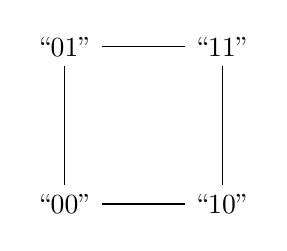
\begin{tikzpicture}
            \node (a) at (0, 0){``00''};
            \node (b) at (0, 2){``01''};
            \node (c) at (2, 0){``10''};
            \node (d) at (2, 2){``11''};
            \draw (a) -- (b) -- (d) -- (c) -- (a);
        \end{tikzpicture}
        
        3-D Hypercube: (on next page)
        
        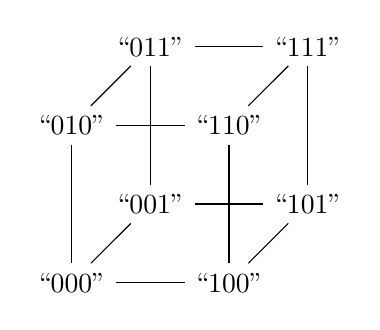
\begin{tikzpicture}
            \node (a) at (0, 0){``000''};
            \node (b) at (2, 0){``100''};
            \node (c) at (2, 2){``110''};
            \node (d) at (0, 2){``010''};
            \node (e) at (1, 1){``001''};
            \node (f) at (3, 1){``101''};
            \node (g) at (3, 3){``111''};
            \node (h) at (1, 3){``011''};
            \draw (a) -- (b) -- (c) -- (d) -- (a);
            \draw (e) -- (f) -- (g) -- (h) -- (e);
            \draw (a) -- (e);
            \draw (b) -- (f);
            \draw (c) -- (g);
            \draw (d) -- (h);
        \end{tikzpicture}
        
        \item We will show inductively that for any $n\geq1$, the $n$ dimensional hypercube can be split into two disjoint sets (which we'll call set $A$ and $B$) of vertices of equal cardinality such that the graph is bipartite.
        
        \textit{Base Case:} When $n=1$, we have two vertices connected by an edge. The graph is obviously bipartite as we can put each vertex in its own group, with no edges within each group, and each group has an equal number of vertices (i.e. one).
        
        \textit{Inductive Hypothesis:} Suppose that for some $n\geq1$, the $n$ dimensional hypercube can be split into two disjoint sets of vertices of equal cardinality (call these two sets $A$ and $B$), such that its graph is bipartite. 
        
        \textit{Inductive Step:} To form the $n+1$ dimensional hypercube, we can take two $n$ dimensional hypercubes and draw an edge between each corresponding vertex. Say the $n$ dimensional hypercube is bipartite with disjoint sets of vertices $A$ and $B$, both with $2^{n-1}$ vertices. Then to form the $n+1$ dimensional hypercube, we create mirrored sets $A'$ and $B'$ of a duplicate $n$ dimensional hypercube such that we only draw additional edges between corresponding vertices in $A$ and $A'$, and between corresponding vertices in $B$ and $B'$. Then we can divide the $n+1$ dimensional hypercube into two sets $A\cup B'$ and $B\cup A'$. There cannot exist an edge within $A$, $B$, $A'$, or $B'$ by the inductive hypothesis, and furthermore there cannot exist an edge between a vertex in $A$ and a vertex in $B'$ (nor between a vertex in $B$ and a vertex in $A'$) by the method in which we constructed and grouped our vertices in the $n+1$ dimensional hypercube. Therefore the $n+1$ dimensional hypercube is also bipartite, and we can split it into two disjoint sets of vertices of equal cardinality ($|A|=|B|=|A'|=|B'|$, therefore $|A\cup B'|=|B\cup A'|$ since all these sets are disjoint). $\square$
    \end{enumerate}
    
    \item
    \begin{enumerate}
        \setlength{\parskip}{8pt}
        \item Let $V$ be the total number of vertices, $E$ the total number of edges, and $F$ the total number of faces. Then since each edge is counted twice for each bordering face, and each face has 3 edges, then we have that $3F=2E$. Then substituting into Euler's formula we have $V=\frac{E}{3}+2$ or $E=3V-6$. The sum of the "charges" is equal to $\sum_v{(6-\text{degree}{(v)})}=6V-2E$, since each edge is counted twice in the sum of the degrees of the vertices. Then combining what we have above we get $6V-2E=6V-2(3V-6)=\boxed{12}$.
        
        \item The charge of a degree 5 vertex is \boxed{1}, and the charge of a degree 6 vertex is \boxed{0}.
        
        \item After discharging all the degree 5 vertices, the only way for a degree 5 vertex to retain a positive remaining charge is for it to be adjacent to at least one other vertex of degree less than or equal to 6 (any vertex of degree $>6$ would have negative charge). Then, under this assumption, the proof follows since either condition (1), (2), or (3) must be true.
        
        \item After discharging, the sum of the charges of all the vertices should remain unchanged, since discharging \textit{transfers} portions of charge from degree 5 vertices to other negatively charged vertices. Thus the total charge must remain 12, and there must exist at least one vertex with positive charge (if all the charges were negative, they wouldn't be able to sum to 12).
        
        Since all degree 5 vertices are "fully" discharged to 0, no degree 5 vertex can have positive charge. The only possible degree of a vertex that goes from negative to positive charge is 7. This is because a degree 7 vertex can receive up to $7\cdot\frac{1}{5}=\frac{7}{5}$ positive charge from surrounding degree 5 vertices, and this is enough to convert its charge of -1 to a positive charge. For any vertex of degree $d>7$, $d\cdot\frac{1}{5}=\frac{d}{5}<|6-d|$, i.e. the surrounding charges from degree 5 vertices is not enough to convert the vertex to a positive degree. Also, degree 6 vertices are unaffected but have 0 charge. Thus the only possible degrees of any positively charged vertex after discharging are \boxed{\text{1, 2, 3, 4, and 7}}.
        
        \item If there exists a degree 7 vertex with positive charge, then it must have \boxed{\text{6 or 7}} adjacent degree 5 vertices, since it's original charge was -1, and it takes at least 6 one-fifth charges to reach a positive charge.
        
        \item Call the degree 7 vertex $a$, and its 7 neighbors $b_1,b_2,b_3,b_4,b_5,b_6,b_7$ in clockwise order. Then, since the graph is triangulated and planar, there must exist an edge between $b_i$ and $b_{i+1}$ for $1\leq i\leq 7$ (since any face consisting of $b_i$, $b_{i+1}$, and $a$ can only have 3 edges, and 2 of the 3 are already drawn) where $i$ and $i+1$ are taken mod 7. Therefore, since at least 6 of the $b_i$ are degree 5, there must exist an edge between two degree 5 vertices, or an edge between a degree 5 vertex and a degree 6 vertex.
        
        \item Let $T$ be any triangulated planar graph. Then from part (a), we know that the total charge of $T$ must be 12. Now, if we "discharge" all degree 5 vertices in $T$, then one of two things can result: (i) there exists a degree 5 vertex with positive charge, or (ii) there exists no degree 5 vertex of positive charge. 
        
        If (i) is true, then by (c) there must exist two degree 5 vertices which are adjacent, satisfying condition (2). 
        
        On the other hand, if (ii) is true, then by (d) there must exist a vertex of degree either 1, 2, 3, 4, or 7. If the vertex has degree 1, 2, 3, 4, condition (1) is satisfied. If the vertex has degree 7, then by parts (e) and (f), we know that there must exist two degree 5 vertices which are adjacent to each other, satisfying condition (2) or condition (3).
        
        Thus we have shown that no matter what either condition (1) or condition (2) or condition (3) will be satisfied for triangulated planar graphs. $\square$
        
    \end{enumerate}
    
\end{enumerate}
\textbf{2.1 Solution.} Suppose we have $v_1,v_2\in V$. Then $(v_1+U)+(v_2+U) = (v_1+v_2)+U$. Now, suppose we have a $v_1'\in V$ such that $v_1+U = v_1'+U$. It follows that $v_1'-v_1\in U$ by Exercise \textbf{1.20}. Therefore we have
\begin{align*}
    (v_1'+U)+(v_2+U) &= (v_1'+v_2+U) \\
                     &= (v_1+v_2)+(v_1'-v_1)+U \\
                     &= (v_1+v_2)+U \\
                     &= (v_1+U)+(v_2+U).
\end{align*}
Notice that the $(v_1'-v_1)$ gets absorbed into $U$ since it is an element of $U$. We can do the same thing for a $v_2'$ such that $v_2'+U=v_2+U$, but the proof is the same due vector space commutativity. Thus, the rule for addition in $V/U$ is well-defined.

\textbf{2.2 Solution.} Since $V/U$ is a vector space endowed with the provided rules of addition and scalar multiplication, we only need to show that $|W|/|U|\subseteq|V|/|U|$, $|W|/|U|$ is nonempty, and that it is closed under addition and scalar multiplication.

Since $|W|/|U|$ is the set $\{w+U\mid w\in W\}$ and $|V|/|U|$ is the set $\{v+U\mid v\in V\}$, it follows that $|W|/|U|\subseteq|V|/|U|$ since $W\sqsubseteq V$ and therefore $|W|\subseteq|V|$.

Next, we know that $|W|/|U|$ must be nonempty since $|W|$ and $|U|$ are nonempty ($|W|$ and $|U|$ are both nonempty since $U\sqsubseteq W\sqsubseteq V$, so both must contain the $0$ vector).

Finally, we show that $W/U$ is closed under addition and scalar multiplication. Since $W$ is a vector space, for any $w_1,w_2\in W$, we know that $w_1+w_2\in W$. Therefore for any $w_1+U,w_2+U\in W/U$, we know that $w_1+w_2+U\in W/U$. Furthermore, for any $w\in W$ and $a\in\mathbb{F}$, we know that $aw\in W$. Therefore for any $w+U\in W/U$, we know that $aw+U\in W/U$. It follows that $W/U$ is closed under both operations.

Thus $W/U\sqsubseteq V/U$.

\textbf{2.3 Solution.} We can see that $\mathbb{R}^3/E_3$ is the space whose underlying set is $\{(x,y,z)+E_3\mid x,y,z\in\mathbb{R}\}$. In other words, it is the collection of all lines parallel to the $z$-axis. Denote the line parallel to the $z$-axis passing through points $(x,y,z)\mid z\in\mathbb{R}$ as $[x,y]$. It follows that there is a 1-to-1 correspondence between $[x,y]\in\mathbb{R}^3/E_3$ and ordered pairs $(x,y)\in\mathbb{R}^2$ given by the isomorphic mapping $\phi:[x,y]\mapsto(x,y)$.

Now we will show that $\phi$ is well-defined. We know there exists a bijection between lines parallel to the $z$-axis in $\mathbb{R}^3/E_3$ and ordered pairs $(x,y)$ in $\mathbb{R}^2$. Now, if we define $[x_1,y_1]+[x_2,y_2] = [x_1+x_2,y_1+y_2]$, then it follows that $\phi([x_1,y_1]+[x_2,y_2]) = \phi([x_1+x_2,y_1+y_2]) = (x_1+x_2,y_1+y_2) = (x_1,y_1)+(x_2,y_2) = \phi([x_1,y_1])+\phi([x_2,y_2])$, so $\phi$ satisfies additivity. Furthermore, if we define $a[x,y] = [ax,ay]$, then it follows that $\phi(a[x,y]) = \phi([ax,ay]) = (ax,ay) = a(x,y) = a\phi([x,y])$, so $\phi$ satisfies homogeneity. Therefore $\phi$ is a bijective homomorphism, and thus a well-defined isomorphism.

\textbf{2.4 Solution.} For any $v_1,v_2\in V$, we have that 
\begin{align*}
    \pi_U(v_1+v_2) &= (v_1+v_2) + U \\
                   &= (v_1+U) + (v_2+U) \\
                   &= \pi_U(v_1) + \pi_U(v_2),
\end{align*}
so $\pi_U$ satisfies additivity.

Furthermore, for any $v\in V$ and $a\in\mathbb{F}$, we have that
\begin{align*}
    \pi_U(av) &= av + U \\
              &= (v+U) + \ldots + (v+U) \text{(where (v+U) appears a times)} \\
              &= a(v+U) \\
              &= a\pi_U(v),
\end{align*}
so $\pi_U$ satisfies homogeneity.

Thus $\pi_U$ is linear.

\textbf{2.5 Solution.} (a) For every coset $[v]\in V/U$, the element $v\in V$ is mapped to $[v]$, i.e. $\pi_U(v)=v+U=[v]$. Therefore $\pi_U$ is surjective. 

For all $u\in|U|$, we have that $\pi_U(u)=u+U=|U|$, since $u\in|U|$ implies $u-0\in|U|$, and therefore $u+U=0+U$, which means that the underlying set of $u+U$ is equivalent to the underlying set of $0+U$, which is just $|U|$.

(b) For every $e\in E$, we have that $\pi_U(e) = e+U$. Then, we have that $\pi_U^{-1}(e+U)$ is the set $\{e+u\mid u\in|U|\}$ for every $e\in E$ (since $\pi_U(\{e+u\mid u\in|U|\}) = \{e+u+U\mid e\in E,u\in U\} = \{e+U\mid e\in E\} = e+U$), which is the same thing as the set $\{e+u\mid e\in E, u\in |U|\}$. It follows that $\pi_U^{-1}(\pi_U(E)) = E+|U|$.

(c) For $E+|U|\sqsubseteq V$, we must have either $E\sqsubseteq V$ or $E\subseteq |U|$. If $E\sqsubseteq V$, then $E+|U|$ is the vector space generated by the union of the generating vectors in $E$ and $|U|$, which must be a subspace of $V$ since both $E$ and $U$ are subspaces of $V$. If $E\subseteq |U|$, then $E+|U|$ is just $U$, which is a subspace of $V$.

\textbf{2.6 Solution.} The quotient space of $V/V$ is just $V$ itself. That is, the underlying set of $V/V$ is $\{v+V\mid v\in V\}$, which is just $|V|$ since for every $v\in V$, $v$ gets absorbed into $V$.

For every $v_1,v_2\in V$, we have that $[v_1]+[v_2]=v_1+v_2+V=|V|$ since $v_1+v_2\in V$. Similarly, for every $v\in V$ and $a\in\mathbb{F}$, we have $a[v]=av+V=|V|$ since $av\in V$.

\textbf{2.7 Solution.} The quotient space $V/U$ consists of the set of all $\{v+U\mid v\in V\}$. Suppose we have some $v\in V$. Then for every $v_i$ for $1\leq i\leq s$, $[v]+[v_i] = (v+U)+(v_i+U) = v+v_i+U = v + U = [v]$ since $v_i\in U$ (it must be, as it's a generator for $U$). Thus the $[v_i]$ are the zero elements of $V/U$.

\textbf{2.8 Solution.} Exercise \textbf{1.30} is essentially the same if we let $T$ be the quotient map $\pi_U:V\to V/U$. That is, we have the equation $\pi_U(v) = [v_0]$ for some given $v_0$. Then solutions to this equation are all of the form $v=v_0+u$ for $u\in U$. It follows that $u\in ker(\pi_U)$ since $\pi_U(u) = u+U = |U|$, which is the zero element of $V/U$. We can check the solutions by plugging in $v$, i.e. $\pi_U(v_0+u) = \pi_U(v_0)+\pi_U(u) = [v_0] + 0 = [v_0]$.

\textbf{2.9 Solution.} Say our bijective function is $f:Hom(V,W)\to Hom(V/U,W)$ with $T\mapsto\widetilde{T}$ for $T\in Hom(V,W)$ and $\widetilde{T}\in Hom(V/U,W)$. We have shown previously that $Hom(V,W)$ is a subspace (and therefore a vector space) of $\mathcal{F}(V,W)$ for vector spaces $V$ and $W$. Then since $V/U$ is a vector space, $Hom(V/U,W)$ is also a vector space.

To show additivity, let $T_1,T_2\in Hom(V,W)$ and $\widetilde{T_1},\widetilde{T_2}\in Hom(V/U,W)$ such that $f(T_1)=\widetilde{T_1}$ and $f(T_2)=\widetilde{T_2}$. It follows that $T_1+T_2\in Hom(V,W)$ and $\widetilde{T_1}+\widetilde{T_2}\in Hom(V/U,W)$. Define $\widetilde{T_1+T_2} = \widetilde{T_1}+\widetilde{T_2}$. Then for every $v\in V$ we have
\begin{align*}
    f(T_1+T_2)(v) &= \widetilde{(T_1+T_2)}(v) \\
                  &= \widetilde{T_1}(v)+\widetilde{T_2}(v) \\
                  &= f(T_1)(v)+f(T_2)(v)
\end{align*}
by vector space properties of $Hom(V,W)$ and $Hom(V/U,W)$, therefore satisfying additivity.

To show homogeneity, let $T\in Hom(V,W)$ and $\widetilde{T}\in Hom(V/U,W)$ with $f(T)=\widetilde{T}$. Also let $a\in\mathbb{F}$. It follows that $aT\in Hom(V,W)$ and $\widetilde{aT}\in Hom(V/U,W)$. Define $\widetilde{aT} = a\widetilde{T}$. Then for every $v\in V$, we have
\begin{align*}
    f(aT)(v) &= \widetilde{aT}(v) \\
             &= a\widetilde{T}(v) \\
             &= af(T)(v)
\end{align*}
by vector space properties of $Hom(V,W)$ and $Hom(V/U,W)$, therefore satisfying homogeneity.

Thus the bijection $T\mapsto\widetilde{T}$ is indeed a homomorphism.

\textbf{2.10 Solution.} By the pushforward corollary, $T\circ\pi_U = \pi_{S(U)}\circ S$. Then, for any $v,v'\in V$ suppose $v'-v\in U$. Then $\pi_U(v') = v+U$. We then get
\begin{align*}
    T(v+U) &= \pi_{S(U)}(S(v')) \\
           &= \pi_{S(U)}(S(v'+v-v)) \\
           &= S(v'+v-v)+S(U) \\
           &= S(v)+S(v'-v)+S(U) \\
           &= S(v)+S(v'-v+U) \\
           &= S(v)+S(U)
\end{align*}
by linearity of $S$. Thus $T$ sends $v+U$ to the coset $S(v)+S(U)$.

\textbf{2.11 Solution.} For the first part, the RHS is the space whose underlying set is $\{v+U\mid T(v)=0, v\in V\}$. The LHS is the space whose underlying set is $\{[v]\mid \widetilde{T}([v])=0, [v]\in V/U\}$. In Theorem \textbf{2.1.6} we defined $\widetilde{T}([v])=T(v)$ for every $[v]\in V/U$. Then we can rewrite the underlying set of the LHS as $\{v+U\mid \widetilde{T}([v])=T(v)=0\}$, which is just the underlying set of the RHS. Therefore $ker(\widetilde{T}) = ker(T)/U$.

Similarly, for the second part, the RHS is the space whose underlying set is $\{T(v)\mid v\in V\}$. The LHS is the space whose underlying set is $\{\widetilde{T}([v])\mid [v]\in V/U\}$. Since $\widetilde{T}([v])=T(v)$ for every $[v]\in V/U$, we can rewrite the set of the LHS as $\{\widetilde{T}([v])\mid v\in V\}$, which is just the underlying set of the RHS. Therefore $ran(\widetilde{T})=ran(T)$.

\textbf{2.12 Solution.} Let $X$ be the set of all sets. Then the relation on $X$ of sets having the same cardinality satisfies (we will write $|S|$ to denote the cardinality of a set $S$):
\begin{itemize}
    \item (reflexivity) For every set $S\in X$, $S\sim S$ since $|S|=|S|$.
    \item (symmetry) For all sets $S_1,S_2\in X$, if $S_1\sim S_2$, then $|S_1|=|S_2|$, so it must be true that $|S_2|=|S_1|$, which implies $S_2\sim S_1$.
    \item (transitivity) For all sets $S_1,S_2,S_3\in X$, if $S_1\sim S_2$ and $S_2\sim S_3$, then $|S_1|=|S_2|=|S_3|$ and thus $S_2\sim S_3$.
\end{itemize}

\textbf{2.13 Solution.} We shall denote $X$ as the set $\mathbb{Z}\times\mathbb{Z}\setminus\{0\}$.

(a) For every $(a,b)\in X$, $(a,b)\sim(a,b)$ since $ab=ab$, satisfying reflexivity. For all $(a,b),(c,d)\in X$, if $(a,b)\sim(c,d)$ then $ad=cb$, or $cb=ad$, which implies $(c,d)\sim(a,b)$, satisfying symmetry. For all $(a,b),(c,d),(e,f)\in X$, if $(a,b)\sim(c,d)$ and $(c,d)\sim(e,f)$ then $ad=cb$ and $cf=ed$. Multiplying the first equation by $f$ and the second by $b$, we get $adf=cbf$ and $cbf=edb$, so $adf=edb$. Multiplying by the multiplicative inverse of $d$ we get $af=eb$, which implies $(a,b)\sim(e,f)$, satisfying transitivity. Thus so $\sim$ is an equivalence relation.

(b) First we show that addition is well-defined. Suppose we have $(a,b),(c,d),(a',b')\in X$ such that $(a,b)\sim(a',b')$. Then $ab'=a'b$. We evaluate $[(a,b)]+[(c,d)]=[(ad+cb,bd)]$ and $[(a',b')]+[(c,d)]=[(a'd+cb',b'd)]$. Then, since
\begin{align*}
    (ad+bc)(b'd) &= adb'd+bcb'd \\
                 &= a'dbd+b'cbd \\
                 &= (a'd+b'c)(bd),
\end{align*}
we deduce that $[(ad+cb,bd)]\sim[(a'd+cb',b'd)]$. Therefore addition is well-defined.

Now we show that multiplication is well-defined. Suppose we have the same $(a,b),(c,d),(a',b') \in X$ from before. Then we evaluate $[(a,b)]\cdot[(c,d)] = [(ac,bd)]$ and $[(a',b')]\cdot[(c,d)] = [(a'c,b'd)]$. Then, since 
\begin{align*}
    (ac)(b'd) &= acb'd \\
              &= a'cbd \\
              &= (a'c)(bd),
\end{align*}
we deduce that $[(ac,bd)]\sim[(a'c,b'd)]$. Therefore multiplication is also well-defined.

(c) First we show that $(X,+)$ is abelian. The additive identity is the equivalence class $[(0,1)]$. For every equivalence class $[(a,b)]$, the additive inverse is $[(-a,b)]$. For all equivalence classes $[(a,b)],[(c,d)],[(e,f)]$, we have $[(a,b)]+([(c,d)]+[(e,f)])=[(adf+bcf+bed,bdf)]=([(a,b)]+[(c,d)])+[(e,f)]$, satisfying associativity. Furthermore, we have $[(a,b)]+[(c,d)]=[(ad+cb,bd)]=[(cb+ad,db)]=[(c,d)]+[(a,b)]$, satisfying commutativity. Therefore $(X,+)$ is an abelian group.

Now, we show that $(X\setminus\{0\},\cdot)$ is abelian. The multiplicative identity is the class $[(a,a)]$. For every equivalence class $[(a,b)]$, the multiplicative identity is $[(b,a)]$. For all equivalence classes $[(a,b)],[(c,d)],[(e,f)]$, we have $[(a,b)]\cdot([(c,d)]\cdot[(e,f)]) = [(ace,bdf)] = ([(a,b)]\cdot[(c,d)])\cdot[(e,f)]$, satisfying associativity. Furthermore, we have $[(a,b)]\cdot[(c,d)] = [(ac,bd)] = [(ca,db)] = [(c,d)]\cdot[(a,b)]$, satisfying commutativity. Therefore $(X\setminus\{0\},\cdot)$ is an abelian group.

Finally, we verify distributivity. For all equivalence classes $[(a,b)],[(c,d)],[(e,f)]$, we have that $[(a,b)]\cdot([(c,d)]+[(e,f)]) = [(a,b)]\cdot[(cf+ed,df)] = [(acf+aed, bdf)] = [(b,b)]\cdot[(acf+aed, bdf)] = [(acfb+aedf,bdfb)] = [(a,b)]\cdot[(c,d)]+[(a,b)]\cdot[(e,f)]$.

Thus the set $X$ with the given operations is a field.

\textbf{2.14 Solution.} For every $a\in X$, $a$ must be in the same element of $P$ as itself, satisfying reflexivity. For every $a,b\in X$, if $a$ and $b$ are in the same element of $P$ then it follows that $b$ and $a$ are in the same element of $P$, satisfying symmetry. For every $a,b,c\in X$, if $a$ and $b$ are in the same element of $P$ and $b$ and $c$ are in the same element of $P$, then it follows that $a$ and $c$ are also in the same element of $P$, satisfying transitivity.

Conversely, if we have an equivalence relation $\sim$ on $X$, then the properties of reflexivity, symmetry, and transitivity guarantee that any element of $X$ must be in a single disjoint subset of $X$ (if, we assume for sake of contradiction that $\exists$ and element that is in more than one disjoint subset, then we can merge those disjoint subsets into one single disjoint subset, and reflexivity, symmetry, and transitivity will still hold).

\textbf{2.15 Solution.} Denote the value of $a_n/b_m$ for a $r\in\mathcal{R}$ as $f_r$ (Note that $f_r$ is a real number). Suppose we have real rational functions $r,s,t\in\mathcal{R}$ such that $r\prec s$. It follows that $0\prec s-r$, so $0 < f_s-f_r=f_s-f_r+f_t-f_t=(f_s+f_t)-(f_r+f_t)$. Then $f_r+f_t < f_s+f_t$, which implies that $r+t\prec s+t$. Similarly, suppose we have real rational functions $r,s\in\mathcal{R}$ such that $0\prec r$ and $0\prec s$. Then we have $0 < f_r$ and $0 < f_s$. Since $\mathbb{R}$ is an ordered field, we know that $0 < f_rf_s$. It follows that $0\prec rs$. Thus $(\mathcal{R},\prec,+,\times)$ is an ordered field.

Let $r(x)=p(x)-q(x)=x-c$. Then $r(x)=\frac{x-c}{1}$, so $f_r=\frac{1}{1}=1>0$. It follows that $0\prec r=p-q$, and therefore $q\prec p$, so the identity polynomial is greater than any constant polynomial using this order.

\textbf{2.16 Solution.} For all endomorphisms $T:\mathcal{R}\to\mathcal{R}$, there exists a unique $p\in\mathcal{R}$ such that $T(r)=p\cdot r$ for all $r\in\mathcal{R}$ (In a way, we are likening the vector space $\mathcal{R}$ over the field $\mathcal{R}$ to the one-dimensional vector space $\mathbb{R}$ over the field $\mathcal{R}$).

\textbf{2.17 Solution.} For every $x\in\mathbb{R}$, $x\sim x$ since $x=x+2\pi(0)$, satisfying reflexivity. For every $x,y\in\mathbb{R}$, if $x\sim y$, then there is an integer $n$ s.t. $y=x+2\pi n$. It follows that $x=y+2\pi(-n)$, and so $y\sim x$, satisfying symmetry. Finally, for every $x,y,z\in\mathbb{R}$, if we have $x\sim y$ and $y\sim z$, then $y=x+2\pi(n)$ and $z=y+2\pi(m)$ for integers $n$ and $m$. It follows that $z=x+2\pi(n+m)$, so $x\sim z$, satisfying transitivity. Thus $\sim$ is an equivalence relation.

Define a function $f:\mathbb{R}/\sim\to[0,2\pi)$ with $f([x])=x$ for $x\in[0,2\pi)$ (note that $[0,2\pi)$ covers the set $\mathbb{R}/\sim$). Then for every $x\in[0,2\pi)$, there exists a $[x]\in\mathbb{R}/\sim$ such that $f([x])=x$, so $f$ is surjective. Furthermore, if we have $x,x'\in[0,2\pi)$ such that $f([x])=f([x'])$. It follows then that $x=f([x])=f([x'])=x'$, so $f$ is injective. Therefore $f$ is bijective.

The mapping $(x,y)\mapsto\theta$ for $(x,y)\in S^1$ and $\theta\in[0,2\pi)$ is a bijection since every point $p$ on the unit circle with origin $o$ is in one-to-one correspondence to the angle $\overline{op}$ makes with the $x$-axis. Then, since there is a bijection between $\mathbb{R}/\sim$ and $[0,2\pi)$, it follows that there is a bijection between $\mathbb{R}/\sim$ and $S^1$.

Proof by counterexample: Let $x=0\in[0,2\pi)$. Then $[0]$ is the same equivalence class as $[2\pi]$. We have $f([0])=0^2=0$ and $f([2\pi])=(2\pi)^2=(2\pi)(2\pi)$. But since $2\pi$ is not an integer, $0\not\sim (2\pi)(2\pi)$, and $f([0])\neq f([2\pi])$. Thus $f([x])=x^2$ is not well-defined.

\textbf{2.18 Solution.} From the universal property of quotient maps \textbf{2.1.6}, we know that $ker(\widetilde{\pi}_W) = ker(\pi_W)/U$ since $U\sqsubseteq V$. Also, since $\pi_W(w) = w+W = W$ for all $w\in W$, $ker(\pi_W) = W$. So we have so far $ker(\widetilde{\pi}_W) = ker(\pi_W)/U = W/U$.

The set $\{w+U\mid w\in W\}$ corresponds to $W/U$ and the set $\{v+U\mid v\in V\}$ corresponds to $V/U$. It follows that $W/U\sqsubseteq V/U$ since $W\sqsubseteq V$ (therefore $|W|\subseteq|V|$) and since $W/U$ is closed under addition and s.m. (if $[w],[w']\in W/U$, then $[w]+[w']=[w+w']\in W/U$, and if $a\in\mathbb{F}$, then $a[w]=[aw]\in W/U$).

Thus we have $ker(\widetilde{\pi}_W) = ker(\pi_W)/U = W/U \sqsubseteq V/U$.

\textbf{2.19 Solution.} By the first isomorphism theorem, $V/ker(T)$ is isomorphic to $ran(T)$, which in this case is just $W$, so $V/ker(T)\cong W$. By the correspondence theorem, since $ker(T)\sqsubseteq V$, the quotient map becomes $\pi:V\to V/ker(T)\cong W$, so $T=\pi$. Then since $U'\to\pi(U')$ is a bijection between subspaces of $V$ containing $ker(T)$ and subspaces of $V/ker(T)\cong W$, we have that the map $U\to T^{-1}(U)$ is a bijection between subspaces of $W$ and subspaces of $V$ containing $ker(T)$.

\textbf{2.20 Solution.} By the correspondence theorem, if we take $W_1 = V/U$ and $W_2 = Z$ for all subspaces $Z\sqsubseteq V/U$, then we have that $W_2\sqsubseteq W_1$ which implies $W_2/W_1 \cong \frac{W_2/U}{W_1/U}$, or $\frac{V/U}{Z} \cong \frac{\frac{V/U}{U}}{Z/U}$. Since $\frac{V/U}{U} = \frac{V/U}{U/U} \cong V/U$, we have $\frac{V/U}{Z} \cong \frac{V/U}{Z/U} \cong \frac{V}{Z}$ by the third isomorphism theorem. Thus every quotient space of $V/U$ is isomorphic to a quotient space of $V$.

\textbf{2.21 Solution.} To show additivity, suppose we have $(u,v),(u',v')\in V\oplus V$. Then we have
\begin{align*}
    T((u,v)+(u',v')) &= T((u+u',v+v')) \\
                    &= ((u+u')cos\theta + (v+v')sin\theta, -(u+u')sin\theta + (v+v')cos\theta) \\
                    &= (ucos\theta + vsin\theta, -usin\theta + vcos\theta) + (u'cos\theta + v'sin\theta, -u'sin\theta + v'cos\theta) \\
                    &= T(u,v) + T(u',v').
\end{align*}

Now we check homogeneity. Suppose we have $(u,v)\in V\oplus V$ and $a\in\mathbb{R}$. Then we have
\begin{align*}
    T(a(u,v)) &= T(au,av) \\
              &= (aucos\theta + avsin\theta, -ausin\theta + avcos\theta) \\
              &= a(ucos\theta + vsin\theta, -usin\theta + vcos\theta) \\
              &= aT(u,v).
\end{align*}

Thus $T$ is linear.
\textbf{2.21 Solution.} Let $T:V \oplus W \to (V/A) \oplus (W/B)$ be the homomorphism defined with the map $(v,w) \mapsto (v+A, w+B)$ for $v \in V$ and $w \in W$. Then $ran(T)$ is just $(V/A) \oplus (W/B)$ and $ker(T)$ is the collection of $(v,w)$ such that $v \in A$ and $w \in B$, or just $A \oplus B$. Then it follows from the First Isomorphism theorem that $(V \oplus W)/(A \oplus B) \cong (V/A) \oplus (W/B)$, and we are done.

\textbf{2.22 Solution.} Since $E_1 \cong E_3$ by the bijective map $(x,0,0) \mapsto (0,0,x)$, we have $E_{1,2} \oplus E_1 \cong E_{1,2} \oplus E_3 \cong \mathbb{R}^3$ by the bijective map $((x,y),z) \mapsto (x,y,z)$.

Since $E_1 \sqsubseteq E_{1,2}$, we know that $E_{1,2} + E_1 = E_{1,2} \cong \mathbb{R}^2$ by the natural mapping $(x,y) \mapsto (x,y)$.

\textbf{2.23 Solution.} To show additivity, suppose we have $(u,v),(u',v')\in V\oplus V$. Then we have
\begin{align*}
    T((u,v)+(u',v')) &= T((u+u',v+v')) \\
                    &= ((u+u')cos\theta + (v+v')sin\theta, -(u+u')sin\theta + (v+v')cos\theta) \\
                    &= (ucos\theta + vsin\theta, -usin\theta + vcos\theta) + (u'cos\theta + v'sin\theta, -u'sin\theta + v'cos\theta) \\
                    &= T(u,v) + T(u',v').
\end{align*}

Now we check homogeneity. Suppose we have $(u,v)\in V\oplus V$ and $a\in\mathbb{R}$. Then we have
\begin{align*}
    T(a(u,v)) &= T(au,av) \\
              &= (aucos\theta + avsin\theta, -ausin\theta + avcos\theta) \\
              &= a(ucos\theta + vsin\theta, -usin\theta + vcos\theta) \\
              &= aT(u,v).
\end{align*}

Thus $T$ is linear.

\textbf{2.24 Solution.} Since $E_{1,2} \cap E_1 = E_1 \neq \{0\}$, there must exist an element in $E_{1,2}+E_1$ that cannot be uniquely expressed by separate vectors in $E_{1,2}$ and $E_1$ from 2.3.9(c). Then since $E_{1,2}+E_1 \sqsubseteq \mathbb{R}^3$, it follows that there exists an element in $\mathbb{R}^3$ that cannot be uniquely expressed. Thus $E_{1,2} \oplus E_1$ is not a direct sum decomposition of $\mathbb{R}^3$ since the codiagonal map is not injective. For example, both $((1,1,0),(0,0,0))$ and $((0,1,0),(1,0,0))$ map to $(1,1,0)$ via the codiagonal map.

We can define a bijective map between $E_{1,2} \oplus E_1$ and $\mathbb{R}^3$ with $((x,y,0),(z,0,0)) \mapsto (x,y,z)$ for $(x,y,0) \in E_{1,2}$ and $(z,0,0) \in E_1$.

\textbf{1.25 Solution.} Suppose we have subspaces $E_1, E_2$, and the collection of all vectors $(x,x)$ for $x \in \mathbb{R}$ (in other words, the subspace of the line $y=x$). These subspaces all intersect pairwise only at the origin. However, they clearly do not form a direct sum decomposition of $\mathbb{R}^2$ since the codiagonal map $((a,0),(0,b),(c,c)) \mapsto (a+c,b+c)$ is not injective. That is, both $((1,0),(0,1),(0,0))$ and $((0,0),(0,0),(1,1))$ map to $(1,1)$.

\textbf{1.26 Solution.} $a \implies b$ direction: Suppose we have a $v \in U_i \cap \sum\limits_{j\neq i}U_j$. WLOG assume $i=1$. Then $v \in U_1$ and $v \in \sum\limits_{j\neq 1}U_j$. From the former it follows that $(v,0,0,\ldots,0) \mapsto v$; from the latter it follows that we can find a $(0,u_2,u_3,\ldots,u_s)$ such that $\sum\limits_{i=2}^s u_i = v$ so that $(0,u_2,u_3,\ldots,u_s) \mapsto v$. Then since (a) implies injectivity of the codiagonal map, we have $(v,0,0,\ldots,0) = (0,u_2,u_3,\ldots,u_s)$. It follows that $v = 0$, concluding the $a \implies b$ direction.

$b \implies a$ direction: The codiagonal map is surjective by definition (for every $u_1+u_2+\ldots+u_s \in U_1+U_2+\ldots+U_s$, we have that $(u_1,u_2,\ldots,u_s)$ maps to it). To prove injectivity, suppose we have $(u_1,u_2,\ldots,u_s)$ and $(u_1',u_2',\ldots,u_s')$ such that $u_1+u_2+\ldots+u_s = u_1'+u_2'+\ldots+u_s'$ through the codiagonal map. Then we have $u_1-u_1' = (u_2'-u_2)+(u_3'-u_3)+\ldots+(u_s'-u_s)$. Since $u_1-u_1' \in U_1$ and $(u_2'u_2)+(u_3'-u_3)+\ldots+(u_s'-u_s) \in \sum\limits_{j\neq 1}U_j$, it follows that both sides of the equation are an element of $U_1 \cap \sum\limits_{j\neq 1}U_j$, which by (b) must be the zero. Then $u_1-u_1' = 0$ and we have $u_1 = u_1'$. Similarly, $u_i = u_i'$ for all $1 \leq i \leq s$. Thus $(u_1,u_2,\ldots,u_s) = (u_1',u_2',\ldots,u_s')$, proving injectivity of the codiagonal map. Thus the codiagonal map is bijective and $U_1 \oplus U_2 \oplus \ldots \oplus U_s$ is a direct sum decomposition of $U_1 + U_2 + \ldots + U_s$.

\textbf{2.27 Solution.} (a) True. $U + E_1$ is the collection of vectors $\{(x,y,0) + (x',0,0) \mid x,y,x' \in \mathbb{R}\}$, which is equivalent to $\{(x,y,0) \mid x,y \in \mathbb{R}\}$, or $E_{1,2}$, which is a subspace of $\mathbb{R}^3$.

(b) True. We can see that $U \cap E_{1,2} = \{(0,0,0)\}$, the zero vector. So by 2.3.9, this is equivalent to $U \oplus E_{1,2}$ being a direct sum decomposition of $\mathbb{R}^3$.

\textbf{2.28 Solution.} Let $\mathbb{F}$ be the field of $U$. Suppose $u_2 = cu_1$ for some non-zero scalar $c \in \mathbb{F}$. Then by definition $span(u_1) = \{au_1 \mid a \in \mathbb{F}\}$ and $span(u_2) = \{acu_1 \mid a \in \mathbb{F}\} = \{bu_1 \mid b \in \mathbb{F}\}$. But then $span(u_1) = span(u_2)$, so by contradiction we know that $u_2 \neq cu_1$ for any non-zero scalar $c \in \mathbb{F}$.

Now, suppose we have a vector $v$ such that $v \in span(u_1)$ and $v \in span(u_2)$. Then we can write $v = c_1u_1$ and $v = c_2u_2$ for scalars $c_1,c_2 \in \mathbb{F}$. It follows that $c_1u_1 = c_2u_2$, and $u_2 = (c_2)^{-1}c_1u_1$. But from before we know that $(c_2)^{-1}c_1$ cannot be non-zero, so it must be 0. Therefore $v = u_2 = 0u_1 = 0$. Then $span(u_1) \cap span(u_2)$ must be $\{0\}$. From 2.3.9, we can deduce that $span(u_1) \oplus span(u_2)$ is a direct sum decomposition of $span(u_1) + span(u_2) = span(u_1,u_2) = U'$, and we are done.

\textbf{2.29 Solution.} Drawing the vectors tip to tail weighted by the coefficients of the dependency relation $(c_1,c_2,\ldots,c_s)$ is equivalent to the linear combination $c_1v_1 + c_2v_2 + \ldots + c_sv_s$. Then by definition of a linearly dependent set, we know that $c_1v_1 + c_2v_2 + \ldots + c_sv_s = 0$. Thus the result is the zero vector, which is equivalent to returning where you started.

\textbf{2.30 Solution.} If we have $a_1v_1 + \ldots + a_sv_s = b_1v_2 + \ldots + b_sv_s$ then we can get $(a_1-b_1)v_1 + \ldots + (a_s-b_s)v_s = 0$. By the definition of linearly independent, it follows that $a_i-b_i = 0$ for each $1 \leq i \leq s$. Therefore $a_i = b_i$ for $1 \leq i \leq s$.

\textbf{2.31 Solution.} Suppose $X = \{x_1,x_2,\ldots,x_s\}$. Then we want to show that the set $\{\delta_{x_i} \mid 1 \leq i \leq s\}$ is a linearly independent generating set. Then let $(c_1,c_2,\ldots,c_s)$ be a list of coefficients with $c_i \in \mathbb{F}$ such that $\sum\limits_{i=1}^s c_i\delta_{x_i} = 0$. Then evaluate the function at each $x_i$ and we get $c_i\delta_{x_i}(x_i) = c_i = 0$ for $1 \leq i \leq s$. It follows that $c_1 = c_2 = \ldots = c_s = 0$, and $\{\delta_x \mid x \in X\}$ is a linearly independent generating set, or basis, for $\mathbb{F}\langle x \rangle$.

\textbf{2.32 Solution.} Suppose $V = U_1 \oplus U_2 \oplus \ldots \oplus U_n$ for some $n \geq 2$ (note that we can also write $V = U_1 + U_2 + \ldots + U_n$ since $U_1 \oplus U_2 \oplus \ldots \oplus U_n$ is a direct sum decomposition of $V$). Then let $T: V \to V$ be the left shift map defined as $(x_1,x_2,\ldots,x_n) \mapsto (x_2,x_3,\ldots,x_n,0)$ for $(x_1,x_2,\ldots,x_n), (x_2,x_3,\ldots,x_n,0) \in U_1+\ldots+U_n$ (here we are defining each one-dimensional subspace $U_i$ as the $i$th coordinate of a vector in $V$). We can see that $ran(T) = U_1 + U_2 + \ldots + U_{n-1}$ and $ker(T) = U_1$. It follows that since $U_1 \in U_1 + U_2 + \ldots + U_{n-1} \cap U_1$ and $U_1 \neq \{0\}$, $ran(T) \oplus ker(T)$ cannot be a direct sum decomposition by 2.3.9b.

\textbf{2.33 Solution.} Let $T: X_1 \times X_2 \to \{f:\{1,2\}\to X_1 \cup X_2 \mid f(1) \in X_1, f(2) \in X_2\}$ be defined with the map $(x_1,x_2) \mapsto f$ where $f$ is defined as $f(1) = x_1$ and $f(2) = x_2$ for $x_1 \in X_1$ and $x_2 \in X_2$. 

To prove injectivity, suppose we have $f,f' \in \{f:\{1,2\}\to X_1 \cup X_2 \mid f(1) \in X_1, f(2) \in X_2\}$ such that $f = f'$. In other words $T(x_1,x_2) = T(x_1',x_2')$ for some $x_1,x_1' \in X_1$ and $x_2,x_2' \in X_2$. It follows that $f$ and $f'$ agree on all points in their domain, so we have $x_1 = f(1) = f'(1) = x_1'$ and $x_2 = f(2) = f'(2) = x_2'$. Thus $(x_1,x_2) = (x_1',x_2')$, proving injectivity.

Now, to show surjectivity, suppose we have any $f \in \{f:\{1,2\}\to X_1 \cup X_2 \mid f(1) \in X_1, f(2) \in X_2\}$. Then suppose $f(1) = x_1$ and $f(2) = x_2$ for some $x_1 \in X_1$ and $x_2 \in X_2$. Then the element $(x_1,x_2) \in X_1 \times X_2$ maps to $f$ by $T$, proving surjectivity.

Thus, since $T$ is both injective and surjective, it is bijective, so there is a bijection between $X_1 \times X_2$ and $\{f:\{1,2\}\to X_1 \cup X_2 \mid f(1) \in X_1, f(2) \in X_2\}$

\textbf{2.34 Solution.} We can define addition and scalar multiplication as coordinate wise for each element in $\prod_{i \in I}V_i$. That is, for each $i \in I$, if we have two "vectors" (or in this case, functions) $f$ and $g$ in $\prod_{i \in I}V_i$ and a scalar $a \in \mathbb{F}$. Then $(f+g)(i) = f(i) + g(i) \in V_i$ and $(af)(i) = af(i) \in V_i$. It follows that $f+g \in \prod_{i \in I}V_i$ and $af \in \prod_{i \in I}V_i$ since the vector space axioms are inherited from each of the $V_i$.

We have shown prior that the free space $\mathbb{F}\langle X \rangle$ is a subspace of the function space $\mathcal{F}(X,\mathbb{F})$. Since $\bigoplus_{i \in I}V_i$ is equivalent to the free space $V\langle I \rangle$ (where we replace field addition with vector addition and field multiplication with scalar multiplication) and furthermore $\prod_{i \in I}V_i$ is equivalent to the function space $\mathcal{F}(I,V)$, we can deduce that $\bigoplus_{i \in I}V_i \sqsubseteq \prod_{i \in I}V_i$.

We use the example of $(V_i)_{i \in \mathbb{N}}$ where each $V_i = \mathbb{F}$. So $\bigoplus_{i \in \mathbb{N}}\mathbb{F}$ is a subspace of $\prod_{i \in \mathbb{N}}\mathbb{F}$. However, since the latter contains the infinite sequence $(1,1,1,\ldots)$ where $f(i) = 1 \in \mathbb{F}$ for every $i \in \mathbb{N}$, whereas the former does not since the direct sum only contains functions with finite support, we indeed have $\bigoplus_{i \in \mathbb{N}}\mathbb{F} \sqsubseteq \prod_{i \in \mathbb{N}}\mathbb{F}$.

\textbf{2.35 Solution.} The codiagonal map $\bigtriangledown$ is surjective by definition. So we want to show injectivity. Suppose we have $v_{\alpha_1} + v_{\alpha_2} + \ldots + v_{\alpha_n} + 0 + \ldots = v_{\alpha_1}' + v_{\alpha_2}' + \ldots + v_{\alpha_n}' + 0 + \ldots$ (where everything vanishes to 0 except for finitely many points $\alpha_i \in \mathbb{N}$) both in the space of $+_{\alpha_i \in \mathbb{N}}E_{\alpha_i}$ such that $v_{\alpha_i},v_{\alpha_i}' \in E_{\alpha_i}$. Then we have $v_{\alpha_1} - v_{\alpha_1}' = (v_{\alpha_2}' - v_{\alpha_2}) + \ldots (v_{\alpha_n}' - v_{\alpha_n})$. Since the RHS is the collection of all sequences that vanish at all but finitely many points and is zero at $\alpha_1$, we know that $v_{\alpha_1} - v_{\alpha_1}' = 0$, so $v_{\alpha_1} = v_{\alpha_1}'$, and similarly each of the $v_{\alpha_i} = v_{\alpha_i}'$. It follows that the codiagonal map is injective, and $\bigoplus_{i \in \mathbb{N}}E_i$ is indeed a direct sum decomposition.

\textbf{2.36 Solution.} To show that $(ie_i)_{i \in \mathbb{N}}$ is a basis for $\mathbb{R}^{\infty}$, we need to show the codiagonal map $\bigtriangledown: \bigoplus_{i \in \mathbb{N}}(span(ie_i)) \to \mathbb{R}^{\infty}$ is injective (note that the map is surjective by definition of $\mathbb{R}^{\infty}$). Suppose we have sequences $(f(1),f(2),\ldots,f(n),0,\ldots) = (a_1,a_2,\ldots,a_n,0,\ldots) = (a_1',a_2',\ldots,a_n',0,\ldots) = (g(1),g(2),\ldots,g(n),0,\ldots)$ both in $\mathbb{R}^{\infty}$ where $a_i \in span(ie_i)$ for $1 \leq i \leq n$ for some natural number $n$ and $f,g$ are functions in the domain of the map. Then $a_i = a_i'$ for $1 \leq i \leq n$, so $f$ and $g$ agree on points of their domain. It follows that $f=g$ and the map is injective. Thus $(ie_i)_{i \in \mathbb{N}}$ is a basis for $\mathbb{R}^{\infty}$.

\textbf{2.37 Solution.} For $T(x,y) = (2x,2y)$, the $T$-invariant subspaces are any subspace of $\mathbb{R}^2$ (scaling a $(x,y)$ by 2 is the same as scaling vector in $\mathbb{R}^2$ by 2, which is just scalar multiplication, which is closed by definition of a vector space).

For $T(x,y) = (2x,y/2)$, the $T$-invariant subspaces are $E_1,E_2,\{0\},$ and $\mathbb{R}^2$.

For $T(x,y) = (y,x)$, the $T$-invariant subspaces are: the subspace underlied by the set of vectors in $y=x$, the subspace underlied by the set of vectors in $y=-x$, $\{0\}$, and $\mathbb{R}^2$.

\textbf{2.38 Solution.} First note that $T(U+W) = \{T(u+w) = T(u) + T(w) \mid u \in U, w \in W\}$ is a subset of the set $U+W = \{u + w \mid u \in U, w \in W\}$ since $T(u) \in U$ and $T(w) \in W$. So $T(u+w) \in U + W$ for every $u \in U$, $w \in W$. Suppose we have $a \in \mathbb{F}$ and $u,u' \in U$, $w,w' \in W$. Then $T((u+w) + (u'+w')) = T(u+u') + T(w+w')$, which is an element of $U+W$ since $u+u' \in U$ and $w+w' \in W$, satisfying additivity. Furthermore $T(a(u+w)) = T(au) + T(aw)$, which is an element of $U+W$ since $au \in U$ and $aw \in W$, satisfying homogeneity. Thus $T(U+W) \sqsubseteq U+W$, so $U+W$ is a $T$-invariant subspace of $V$.

Now we show the second part. Since $T(U) \sqsubseteq U$ and $T(W) \sqsubseteq W$, we know that, respectively, for any vector $u \in U$, $T(u) \in \{v \mid v \in U\}$ and for any vector $w \in W$, $T(w) \in \{v \mid v \in W\}$. Therefore for any vector $v' \in U \cap W$, we have that $T(v') \in \{v \mid v \in U, v \in W\} = U \cap W$. It follows that $T(U \cap W)$ is a subset of $U \cap W$. Then suppose we have $v,v' \in U \cap W$ and $a \in \mathbb{F}$ such that $T(v),T(v') \in T(U \cap W)$. We want to show that $T(U \cap W)$ is closed under vector addition and scalar multiplication.

If $T(v), T(v') \in T(U \cap W)$, then by linearity of $T$, we have $T(v) + T(v') = T(v + v')$ is also in $T(U \cap W)$ since $v+v' \in U \cap W$ (this follows from vector space properties of $U \cap W$, which we have shown previously to be a vector subspace of $V$). It follows that $T(U \cap W)$ is closed under addition.

IF $T(v) \in T(U \cap W)$, then by linearity of $T$, we have $aT(v) = T(av)$ is also in $T(U \cap W)$ since $av \in U \cap W$ (again, this follows from vector space properties of $U \cap W$). It follows that $T(U \cap W)$ is closed under scalar multiplication.

Thus we have shown that $T(U \cap W) \sqsubseteq U \cap W$ is a $T$-invariant subspace.

\textbf{2.39 Solution.} Suppose we have any sequence $(u_1,\ldots,u_n) \in U_1 \oplus \ldots \oplus U_n$ where $u_i \in U_i$ for $1 \leq i \leq n$. Then we will evaluate the LHS and RHS at $(u_1,\ldots,u_n)$ separately and show that they are equal.

The LHS becomes:
\begin{align*}
    T(\bigtriangledown(u_1,\ldots,u_n) &= T(u_1 + \ldots + u_n) \\
                                       &= T(u_1) + \ldots + T(u_n)
\end{align*}
by linearity of $T$.

The RHS becomes:
\begin{align*}
    \bigtriangledown(T\mid_{U_1} \oplus \ldots \oplus T\mid_{U_n}(u_1,\ldots,u_n)) &= \bigtriangledown(T\mid_{U_1}(u_1) + \ldots + T\mid_{U_n}(u_n)) \\
                                 &= T\mid_{U_1}(u_1) + \ldots + T\mid_{U_n}(u_n) \\
                                 &= T(u_1) + \ldots + T(u_n)
\end{align*}
since both $T\mid_{U_1}\oplus\ldots\oplus T\mid_{U_n}$ and $T$ are linear and since $T\mid_{U_i}(u_i) = T(u_i)$ when $u_i \in U_i$.

Thus the LHS and RHS are equal and we are done.

\textbf{2.40 Solution.} We show that $P$ satisfies reflexivity, antisymmetry, and transitivity. For every subset $S$ of $\mathbb{R}^2$, it is clear that $S\subseteq S$ since $S=S$, satisfying reflexivity. For subsets $S_1,S_2\in\mathbb{R}^2$, if $S_1\subseteq S_2$ and $S_2\subseteq S_1$, then every element that is in $S_1$ is in $S_2$ and vice versa, which is equivalent to $S_1=S_2$, satisfying antisymmetry. For subsets $S_1,S_2,S_3\in\mathbb{R}^2$, if we have $S_1\subseteq S_2$ and $S_2\subseteq S_3$, then any element that is in $S_1$ must be in $S_2$ and therefore in $S_3$, so it follows that $S_1\subseteq S_3$, satisfying transitivity. Therefore $P$ is partially ordered by inclusion. 

For every chain of $P$, we can find an upper bound in $P$ by taking the union of the subsets in the chain. This union set is necessarily in $P$ since the union of an arbitrary number of subsets of a set each with $\leq n$ elements must also be a subset with $\leq n$ elements.

To show any set with $n$ elements is a maximal element in $P$, we assume for sake of contradiction that there exists a set $S$ with $n$ elements that is not a maximal element of $P$. Then there exists an element of $P$ that is strictly greater than $S$. In other words, there exists another set $S'$ with $S\subset S'$. But this means that $S'$ contains every element in $S$ plus at least one element not in $S$, and $S'$ would have at least $n+1$ elements, so it cannot be in $P$, a contradiction.

\textbf{2.41 Solution.} There exists no element (set) in $S$ that is a strict subset of $\{d,o\}$, since none of $\{d\}, \{o\}, \{\}$ are in $S$. Thus $\{d,o\}$ is minimal in $S$.

There exists no element (set) in $S$ that is a strict superset of $\{g,o,a,d\}$, since no set in $S$ contains $g,o,a,d$, and at least one other element. Thus $\{g,o,a,d\}$ is maximal in $S$.

The set $\{d,o,g\}$ is not minimal since $\{d,o\}\subset\{d,o,g\}$. It is also not maximal since $\{d,o,g\}\subset\{g,o,a,d\}$.

We can see that $\{o,a,f\}$ is minimal since no element in $S$ is a strict subset of $\{o,a,f\}$. It is also maximal since no element in $S$ is a strict superset of $\{o,a,f\}$. Thus $\{o,a,f\}$ is both minimal and maximal in $S$.

\textbf{2.42 Solution.} By the complementary subspaces theorem, we can find a subspace $U'$ of $V$ such that $U\oplus U' = V$ (note that, if $U$ were not a strict subspace of $V$, then $U = V$ and we can just define $\overline{T} = T$). Then for every $v\in V$, we can write $v = u + u'$ for unique $u\in U$ and $u'\in U'$. Now, we define $\overline{T}(v) = T(u)$ for every $v\in V$ (essentially, $\overline{T}$ projects $v$ onto $T(u)$ and "eats" $u'$). 

To show additivity, let $v_1,v_2\in V$, $u_1,u_2\in U$, and $u_1',u_2'\in U'$ such that $v_1 = u_1 + u_1'$ and $v_2 = u_2 + u_2'$. Since $v_1 + v_2 = (u_1 + u_2) + (u_1' + u_2')$ with $u_1 + u_2\in U$ and $u_1' + u_2'\in U'$ (both $U$ and $U'$ are subspaces), it follows that $\overline{T}(v_1+v_2) = T(u_1 + u_2) = T(u_1) + T(u_2) = \overline{T}(v_1) + \overline{T}(v_2$ by linearity of $T$.

To show homogeneity, let let $v\in V$, $u\in U$, $u'\in U'$, and $a\in\mathbb{F}$ such that $v = u + u'$. Since $av = a(u + u') = au + au'$ with $au\in U$ and $au'\in U'$ (both $U$ and $U'$ are subspaces), it follows that $\overline{T}(av) = T(au) = aT(u) = a\overline{T}(v)$ by linearity of $T$.

Thus $T$ extends to $\overline{T}\in Hom(V,W)$.

\textbf{2.43 Solution.} For each $f$ with finite support in $\bigoplus_{k \in I}V_k$ with $f(i) = v_i \in V_i$ for $i \in I$, we can define $\bigoplus_{k \in I}T_i$ with the mapping $f \mapsto g$ for a $g$ with finite support in $\bigoplus_{k \in I}W_k$ such that $g(i) = T_i(v_i) \in W_i$ for $i \in I$. 

It is easy to verify that the diagrams commute. For example, for the first diagram, suppose we have a function/sequence $(\ldots,0,v_1,\ldots,v_s,0,\ldots)$. Then $T_i \circ \pi_{V_i}$ sends it to $v_i$ and then to $T(v_i)$, and $\pi_{W_i} \circ \bigoplus_{k \in I}T_i$ sends it to $(\ldots,0,T(v_1),\ldots,T(v_s),0,\ldots)$ and then to $T(v_i)$, so the first diagram commutes.

Similarly for the second diagram, suppose we have a vector $v_i \in V_i$. Then $\bigoplus_{k \in I}T_i \circ j_{V_i}$ sends it to $(\ldots,0,v_i,0,\ldots)$ and then $(\ldots,0,T(v_i),0,\ldots)$ and $j_{W_i} \circ T_i$ sends it to $T(v_i)$ and then to $(\ldots,0,T(v_i),0,\ldots)$, so the second diagram commutes as well.

\textbf{2.44 Solution.} Suppose we have a $v_i \in V_i$ for every $i \in I$. Then from $j_{W_i} \circ T_i = S \circ j_{V_i}$ we have $(\ldots,0,T_i(v_i),0,\ldots) = j_{W_i}(T_i(v_i)) = S(j_{V_i}(v_i)) = S(\ldots,0,v_i,0,\ldots)$ for every $i \in I$ (where $v_i$ and $T_i(v_i)$ have corresponding indices).

Now, suppose we have any function/sequence $f$ in the domain of $S$ (which, by definition, is the same domain as $\bigoplus_{k \in I}T_k$). Then $f$ can be written as $(\ldots,0,v_{k_1},\ldots,v_{k_s},0,\ldots)$ where $k_l \in I$ and $v_{k_l} \in V_{k_l}$ for $1 \leq l \leq s$. Then since $S$ is given to be a homomorphism, and since we showed $S(\ldots,0,v_i,0,\ldots) = (\ldots,0,T_i(v_i),0,\ldots)$ for every $i \in I$, we have
\begin{align*}
S(\ldots,0,v_{k_1},\ldots,v_{k_s},0,\ldots) &= S(\ldots,0,v_{k_1},0,\ldots) + \ldots + S(\ldots,0,v_{k_s},0,\ldots) \\
&= (\ldots,0,T_{k_1}(v_{k_1}),0,\ldots) + \ldots + (\ldots,0,T_{k_s}(v_{k_s}),0,\ldots) \\
&= (\ldots,0,T_{k_1}(v_{k_1}),\ldots,T_{k_s}(v_{k_s}),0,\ldots)
\end{align*}
Thus $S$ and $\bigoplus_{k \in I}T_k$ agree at every point in their domain, thus $S = \bigoplus_{k \in I}T_k$.

\textbf{2.45 Solution.} False. Suppose we have a function $f \in \bigoplus_{k \in I}V_k$ given by the sequence $(\ldots,0,v_{k_1},\ldots,v_{k_s},0,\ldots)$ where $k_l \in I$ and $v_{k_l} \in V_{k_l}$ for $1 \leq l \leq s$ (where more than one of the $v_{k_l}$'s are nonzero). Then $j_{V_i}(\pi_{W_i}(f)) = (\ldots,0,v_i,0,\ldots) \neq (\ldots,0,v_{k_1},\ldots,v_{k_s},0,\ldots)$, which means that $j_{V_i} \circ \pi_{W_i} \neq Id_{\bigoplus_{k \in I}V_k}$, and therefore the diagram does not commute.
\textbf{5.1 Solution.} Suppose we have objects $A, B \in Alg_{\mathbb{F}}$, and functions $f \in Hom_{Alg_{\mathbb{F}}}(A, B)$ and $g \in Hom_{Alg_{\mathbb{F}}}(B, A)$. Then define $Id_A : A \to A$ as the function $Id_A(a) = a$ for every $a \in |A|$. It follows that for every $a \in |A|$, we have $(f \circ Id_A)(a) = f(Id_A(a)) = f(a)$, and for every $b \in |B|$ we also have $(Id_A \circ g)(b) = Id_A(g(b)) = g(b)$, since $g(b) \in |A|$. Therefore $Alg_{\mathbb{F}}$ satisfies left and right unit axioms.

Now, suppose we have objects $A, B, C, D \in Alg_{\mathbb{F}}$ and functions $f_1 \in Hom_{Alg_{\mathbb{F}}}(A, B)$, $f_2 \in Hom_{Alg_{\mathbb{F}}}(B, C)$, and $f_3 \in Hom_{Alg_{\mathbb{F}}}(C, D)$. For every $a \in |A|$, let $f_1(a) = b$ for some $b \in |B|$, and let $f_2(b) = c$ for some $c \in |C|$, and let $f_3(c) = d$ for some $d \in |D|$. Then we have that $(f_3 \circ f_2)$ sends $b$ to $d$, and similarly $(f_2 \circ f_1)$ sends $a$ to $c$. It follows that for every $a \in |A|$
\begin{align*}
((f_3 \circ f_2) \circ f_1)(a) &= (f_3 \circ f_2)(b) \\
    &= d \\
    &= f_3(c) \\
    &= f_3 \circ (f_2 \circ f_1)(a).
\end{align*}
So since $(f_3 \circ f_2) \circ f_1$ and $f_3 \circ (f_2 \circ f_1)$ agree on every point in their domain, i.e. $A$, composition is associative.

Thus $Alg_{\mathbb{F}}$ satisfies all the category axioms.

\textbf{5.2 Solution.} For $\bf{C_1}$: The identity is simply $Id_A : A \to A$ since $(Id_A \circ Id_A)(A) = Id_A(A)$, satisfying both left and right unit axioms. Associativity follows as well since $(Id_A \circ Id_A) \circ Id_A = Id_A \circ Id_A = Id_A \circ (Id_A \circ Id_A)$.

For $\bf{C_2}$: Using the same logic from $\bf{C_1}$, the identities on $A$ and $B$ satisfy left and right unit and associtivity axioms. So we only need to check unit and associtivity for the morphism $f: A \to B$. We have $(f \circ Id_A)(A) = f(Id_A(A)) = f(A)$ and $(Id_B \circ f)(A) = Id_B(f(A)) = f(A)$, satisfying unit axioms. Furthermore, since $f$ can only compose with $Id_A$ and $Id_B$, associativity easily follows for all cases.

For $\bf{C_3}$: Using the same reasoning from the first two parts, unit and associtivity axioms can be verified for all pairs and individuals objects in $\bf{C_3}$. Therefore we only need to verify associativity of morphisms consisting of 3 objects. Let $f: A \to B$, $g: B \to C$, $h: C \to A$. Then we have $((h \circ g) \circ f)(A) = (h \circ g)(B) = h(g(B)) = h(C) = A = h(C) = h((g \circ f)(A)) = (h \circ (g \circ f))(A)$, satisfying associativity. Thus $\bf{C_3}$ is also a valid category.

\textbf{5.3 Solution.} Suppose we have objects $A, B \in Ob(\bf{C})$ with $g: A \to B$. Also suppose that $F(A), F(B) \in Ob(\bf{D})$. We have that $F$ takes the diagram $A \to B$ to $F(A) \to F(B)$, converting $g$ to $F(g): F(A) \to F(B)$. Since $g$ is an isomorphism, we can apply $F$ to the diagram $B \to A$ obtaining $F(B) \to F(A)$, converting $g^{-1}$ to $F(g^{-1})$. It follows that the inverse of $F(g)$ exists and is $F(g^{-1})$ since the their composition results in the identities, i.e. $(F(g) \circ F(g^{-1}))(F(B)) = F(B)$ and $(F(g^{-1}) \circ F(g))(F(A)) = F(A)$. Thus $F(g)$ is an isomorphism in $\bf{D}$.

\textbf{5.4 Solution.} By definition of covariant functors, all objects and arrows in a commutative diagram of $\bf{D}$ get converted by $G$ to corresponding objects and arrows in $\bf{E}$ such that the diagram in $\bf{E}$ commutes and the arrows point in the same direction. Similarly, all objects and arrows in $\bf{C}$ get converted by $F$ to corresponding objects and arrows in $\bf{D}$ such that the corresponding diagram commutes and the arrows maintain their direction. Therefore if we have any commutative diagram in $\bf{C}$, and we apply the composition $G \circ F$, we will be guaranteed to obtain a commutative diagram with arrows in the same direction in $\bf{E}$. Thus $G \circ F$ is also a covariant functor.

\textbf{5.5 Solution.} For every $X \in \bf{Set}$ and $g \in V \langle X \rangle$, we have that $Free_V(Id_X)(g) = f \circ Id_X = g$, satisfying the identity axiom.

Now suppose we have $X, Y, Z \in \bf{Set}$ and $f: X \to Y$ and $g: Y \to Z$. Then after applying $Free_V$, we get $Free_V(g)$ a function that takes $h \in V \langle Z \rangle$ and sends it to $h \circ g \in V \langle Y \rangle$, and we also get $Free_V(f)$ a function that takes a $h \circ g \in V \langle Y \rangle$ to a function $h \circ g \circ f \in V \langle X \rangle$. Then by composing $Free_V(f) \circ Free_V(g)$ we obtain a function that takes $h \in V \langle Z \rangle$ to $h \circ g \circ f \in V \langle X \rangle$, which is equivalent to $free_V(g \circ f)$ since $g \circ f$ takes $X$ to $Z$. Thus $Free_V$ is indeed a contravariant functor.

\textbf{5.6 Solution.} For every set $X$, the function given by $P(Id_X)$ sends subsets of $X$ to themselves. This is the same as the function given by $Id_{P(X)}$, which sends elements of $P(X)$, subsets of $X$, to themselves. Thus the identity axiom holds for the power set functor.

Suppose we have sets $X, Y, Z$ with set functions $f: X \to Y$ and $g: Y \to Z$. It follows that $P(f)$ sends subsets of $X$ to subsets of $Y$, which are then sent to subsets of $Z$ via $P(g)$. It follows that the composition $P(g) \circ P(f)$ is equivalent to the function $P(g \circ f)$, which sends subsets of its domain $X$ to corresponding subsets of its codomain $Z$. Thus the power set functor is covariant.

The inverse power set functor is essentially the contravariant functor equivalent of the power set functor. It is easy to see that it satisfies all the axioms if we reverse the roles of $X, Y, Z$. That is, $\bf{P^{-1}}$ is also a functor.

\textbf{5.7 Solution.} True. We proved this result in Exercise 5.3.

\textbf{5.8 Solution.} Suppose we have a functor $F: \bf{C} \to \bf{D}$ that is full and faithful. Then there exists a bijection between $Hom_{\bf{C}}(X, Y)$ and $Hom_{\bf{D}}(F(X), F(Y))$ for every $X \in \bf{C}$ and $Y \in \bf{D}$. WLOG, fix $X$ and $Y$.

For the first direction, suppose $F(X)$ and $F(Y)$ are isomorphic in $\bf{D}$. Then there exists functions $F(f): F(X) \to F(Y)$ and $F(f^{-1}): F(Y) \to F(X)$ such that $F(f) \circ F(f^{-1}) = Id_{F(Y)}$ and $F(f^{-1}) \circ F(f) = Id_{F(X)}$. Then since there is a bijection between $Hom_{\bf{C}}(X, Y)$ and $Hom_{\bf{D}}(F(X)$, we know there must exist unique corresponding functions $f: X \to Y$ and $f^{-1}: Y \to X$ such that $f \circ f^{-1} = Id_Y$ and $f^{-1} \circ f = Id_X$. It follows that $X$ and $Y$ are isomorphic in $\bf{C}$.

For the converse, suppose $X$ and $Y$ are isomorphic in $\bf{C}$. Then there exists functions $f: X \to Y$ and $f^{-1}: Y \to X$ such that $f \circ f^{-1} = Id_Y$ and $f^{-1} \circ f = Id_X$. Then since there is a bijection between $Hom_{\bf{C}}(X, Y)$ and $Hom_{\bf{D}}(F(X)$, we know there must exist unique corresponding functions $F(f): F(X) \to F(Y)$ and $F(f^{-1}): F(Y) \to F(X)$ such that $F(f) \circ F(f^{-1}) = Id_{F(Y)}$ and $F(f^{-1}) \circ F(f) = Id_{F(X)}$. It follows that $F(X)$ and $F(Y)$ are isomorphic in $\bf{D}$.

\textbf{5.9 Solution.} Since $X, Y \in Ob(\bf{A})$ satisfy $F(X)$ is isomorphic to $F(Y)$, we have from proposition 5.2.3 that $X$ must be isomorphic to $Y$ since $F$ is a full and faithful functor.

\textbf{5.10 Solution.} %Ab -> Grp is actually full as well, since abelian group morphisms do not impose the extra condition of commutativity, so all abelian group morphisms are group morphisms
It is easy to see that the functor $F: \bf{Ab} \to \bf{Grp}$ is faithful, since every abelian group is a group. Therefore we can send each abelian group to the corresponding group that shares its underlying set, and we can send each abelian group homomorphism to itself by forgetting the axiom of commutativity.

However, $F$ is not full, since there can exist non-abelian groups that do not satisfy commutativity which do not have corresponding objects or morphisms in $\bf{Ab}$.

Thus $\bf{Ab} \to \bf{Grp}$ is faithful but not full.

\textbf{5.11 Solution.} True. All forgetful functors are faithful (here we are mapping each group homomorphism to its underlying function on sets, so it's one to one).

False. Since there exist sets which do not uphold the axioms of a group, we can construct a function on these non-group-conforming sets and it (the function) won't have a corresponding morphism in $\bf{Grp}$.

\textbf{5.12 Solution.} Suppose we have objects $U, U' \in \bf{C}$ and $V, V' \in \bf{D}$ such that we have the morphism $f: (U,V) \to (U',V')$ in $\bf{C} \times \bf{D}$. Then define the forgetful bifunctor $F: \bf{C} \times \bf{D} \to \bf{C}$ that sends ("projects" onto its component in $\bf{C}$) each object $(U,V)$ to $U$, and also sends morphisms of the form $(U,V) \to (U',V')$ to the morphism $U \to U'$. Thus we have a bifunctor $F$ that projects the product category $\bf{C} \times \bf{D}$ onto its component $\bf{C}$.
\section{Homework 7}

Sundry: I worked alone.

\begin{enumerate}
    \item \begin{enumerate}
        \item \begin{enumerate}
            \item Yes. $f(x) = 0.00001x$ is a bijection between $\mathbb{R}$ and $\mathbb{R}$ because for every $b \in \mathbb{R}$ (the codomain), there exists a \textit{unique} $a \in \mathbb{R}$ (the domain) with $a = 100000b$.
            
            \item No. There exists no such $a \in \mathbb{Z} \cup \{\pi\}$ such that $f(a) = \frac{1}{3}$ (if there were, we could find either an integer $x$ or $\pi$ that equals $\frac{10^5}{3}$, but we can't). Thus the function is not surjective on the given domain and codomain, so it can't be a bijection.
        \end{enumerate}
        
        \item \begin{enumerate}
            \item No. Let $p = 3$, then for both $x = 4, 5 \in \mathbb{N} \setminus \{0\}$, we have $f(4) = 3$ and $f(5) = 3$, so $f$ is not injective, and cannot be bijective either.
            
            \item Yes. Each value $x \in \{\frac{p+1}{2}, \ldots p\}$ maps to $p - x \in \{0, \ldots, \frac{p-1}{2}\}$ through the function $f$. In particular, it is easy to see injectivity and surjectivity of $f$ with the mapping $x \mapsto p - x$. It follows that we have a bijection.
        \end{enumerate}
        
        \item This function is injective, but not surjective. That is, there is no element in $D$ that maps to the element $\{\}$ in the power set of $D$.
        
        \item Yes. After shuffling the digits, we still have exactly 10 distinct digits 0 through 9. So taking the $i+1^{\text{st}}$ digit of $X'$ will always result in distinct digit for distinct $i$ (injectivity). Also, since the cardinality of the domain is 10, we know that every element in the codomain gets hit (surjectivity). Thus bijectivity follows.
    \end{enumerate}
    
    \item \begin{enumerate} 
        \item Countable. Since $A$ and $B$ are countable, we can draw a bijection between the two and the set of $\mathbb{N}$. Then we can draw another bijection between $\mathbb{N} \times \mathbb{N}$ and $\mathbb{N}$ by ``snaking'' through the first quadrant of the xy-plane. In particular, we define a bijective mapping:
        \begin{align*}
            0 &\mapsto (0,0) \\
            1 &\mapsto (1,0) \\
            2 &\mapsto (0,1) \\
            3 &\mapsto (0,2) \\
            4 &\mapsto (1,1) \\
            5 &\mapsto (2,0) \\
            &\vdots
        \end{align*}
        which I was too lazy to draw up in tikz.
        
        \item Sometimes Countable, Sometimes Uncountable. Example of Countable: Let all the $B_i = \mathbb{N}$, then their union is $\mathbb{N}$, which is countable. Example of Uncountable: Let $B_i$ for $i \in \mathbb{N}$ be the set of all $i$ digit decimals in $[0,1)$. So $B_1$ would be $\{0.0, 0.1, 0.2, \ldots, 0.9\}$, and $B_2$ would be $\{0.00, 0.01, 0.02, \ldots, 0.99\}$. Then their union would be all the real numbers from 0 to 1, which is uncountably infinite.
        
        \item Uncountable. We prove with a diagonalization argument. Suppose our set is countable. Then we can enumerate every non-decreasing function $f$ in a table, e.g.:
        \[
        \begin{tabular}{c|cccc}
            $x,f(x)$ & $f_1$ & $f_2$ & $f_3$ & \ldots \\
            \hline
            0 & \bf{1} & 0 & 3 & \ldots \\
            1 & 2 & \bf{5} & 3 & \ldots \\
            2 & 4 & 7 & \bf{4} & \ldots \\
            \vdots & \vdots & \vdots & \vdots
        \end{tabular}
        \]
        Notice that we cannot just add 1 to every element along the diagonal to produce another non-decreasing function from $\mathbb{N}$ to $\mathbb{N}$. Instead, we will add all the preceding elements of the diagonal to the next element. That is, in the example above we'd replace $(1, 5, 4, \ldots)$ with $(1, 6, 10, \ldots)$. This way we will obtain a non-decreasing function that differs from all of the $f_i$ at input $i$, contradicting countability. It follows that our set is uncountable.
        
        \item Countably infinite. We can represent each non-increasing function as a list of natural numbers (where the indeces are the inputs from $\mathbb{N}$ and the values are the outputs of $f$ also in $\mathbb{N}$). Then we can order them by coordinate from least to greatest. That is, we can obtain the mapping:
        \begin{align*}
            0 &\mapsto (0, 0, 0, \ldots) \\
            1 &\mapsto (1, 0, 0, \ldots) \\
            2 &\mapsto (1, 1, 0, \ldots) \\
            3 &\mapsto (1, 1, 1, \ldots) \\
              &\vdots \\
            n &\mapsto (2, 0, 0, \ldots) \\
              &\vdots
        \end{align*}
        where $n \in \mathbb{N}$. Thus we have a bijection between our set and $\mathbb{N}$, so it must be countably infinite.
        
        \item Uncountably infinite. We will construct an injection from $\mathcal{P}(\mathbb{N})$ to the set of all bijective functions from $\mathbb{N}$ to $\mathbb{N}$, from which we can deduce that our set is a superset of an uncountable set, and therefore uncountable itself. For every set $\{a_0, a_1, \ldots, a_k\}$ in $\mathcal{P}(\mathbb{N})$ where the $a_i$ are in $\mathbb{N}$, map it to the bijective function $f: \mathbb{N} \to \mathbb{N}$ defined as $f(x) = x$ if $x \not\in \{a_0, a_1, \ldots, a_k\}$ and $f(a_i) = a_{k - i}$ for $a_i \in \{a_0, a_1, \ldots, a_k\}$. It follows that the set of all bijective functions from $\mathbb{N}$ to $\mathbb{N}$ is at least as big as the power set of $\mathbb{N}$, which is uncountable. Therefore our set is uncountable.
      
    \end{enumerate}
    
    \item \begin{enumerate}
        \item Impossible. Suppose for sake of contradiction that such a program $P$ exists. Then we can construct the program:
        \begin{verbatim}
            def is_halt(F, x):
                def P'():
                    bool = False
                    outputs = (list of all return/print values of F)
                    for y in outputs:
                        bool = bool or P(F, x, o)
                    return bool
                return P'()
        \end{verbatim}
        which successfully tells whether any given program $F$ halts on a given input $x$. But then we have a contradiction, since this solve the halting problem, which is unsolvable. Thus $P$ cannot exist.
        
        \item Impossible. Suppose for sake of contradiction that such a program $P$ exists. Then for any program $F$ and given input $x$, let $G$ be the program constructed as follows:
        \begin{verbatim}
            def G(a):
                if a == x:
                    return something
                'body of F'
        \end{verbatim}
        Then $G$ halts on the same inputs as $F$ does for all inputs except for $x$, for which $G$ certainly halts and $F$ may or may not halt. Now, we can construct the program is\_halt:
        \begin{verbatim}
            def is_halt(F, x):
                def G(a):
                    ...
                return P(F, G)
        \end{verbatim}
        This function will return true is $F$ halts on $x$ and false otherwise, thus solving the halting problem, a contradiction.
    \end{enumerate}
    
    \item \begin{enumerate}
        \item Since there are $n$ states and $k$ instructions, there can be up to $nk$ total iterations before the machine repeats a computation.
        
        \item For any positive integers $n, k$, it is clear that $2n^2k^2 > nk$, so if the algorithm is still running after $2n^2k^2$ iterations, a computation must have been repeated. But this means the same instruction was given the exact same input, which will result in a loop.
        
        \item Plug in $x$ to $i_0$ and keep track of all pairs of inputs and instructions. If at some point before there are more than $nk$ iterations, the program halts, i.e. $j_l \geq k$ for some $l < nk$, then we know that the program halts. Otherwise, it will loop indefinitely. This does not contradict the undecidability of the halting problem, since this particular instance assume we have knowledge of the values of $n$ and $k$, whereas in the traditional halting problem, we do not know these values, so we cannot construct a test\_halt function without these values.
    \end{enumerate}
    
    \item \begin{enumerate}
        \item We have 10 options for each of the four categories, for a total of $10^4 = 10000$ possible distinct outfits.
        
        \item Since there are 10 in each category, we have $\binom{4}{2}10^2 = 600$ possible distinct outfits if we wear exactly two categories.
        
        \item We have $10 \cdot 9 \cdot 8 \cdot 7 = 5040$ ways to hang 4 of out 10 hats in a row.
        
        \item We have the binomial $\binom{10}{4} = 210$ ways to pack 4 hats for travels. This is equivalent to $\frac{10 \cdot 9 \cdot 8 \cdot 7}{4 \cdot 3 \cdot 2 \cdot 1} = \frac{5040}{24}$, as we are simply correcting for overcounting with regards to order.
        
        \item This is equivalent to $\binom{5}{2} = 10$ distinct sets of three hats, since we have 3 hats and 2 `markers' (stars and bars? bins and balls? idk what you guys call it).
    \end{enumerate}
\end{enumerate}
\section{Homework 8}
Sundry: I worked alone.

\begin{enumerate}
    \item \begin{enumerate}
        \item $\binom{n+k}{k}$ or $\binom{n+k}{n}$
        
        \item There are $\binom{52}{13}$ different bridge hands, and $\binom{48}{13}$ different bridge hands that contain no aces, and $\binom{48}{9}$ different bridge hands that contain all four aces, and $\binom{13}{6}\binom{46}{7}$ that contain exactly six spades.
        
        \item $\frac{102!}{2^{52}}$.
        
        \item $\frac{2^{99}}{2} = 2^{98}$.
        
        \item There are $7! = 5040$ anagrams of FLORIDA, there are $\frac{6!}{3!}$ anagrams of ALASKA, there are $\frac{7!}{4!}$ anagrams of ALABAMA, and $\frac{7!}{2!2!}$ anagrams of MONTANA.
        
        \item For part (1), there are $5!$ such anagrams. For part (2), there are $\frac{6!}{2} = 360$ such anagrams.
        
        \item $27^9$.
        
        \item $\binom{7}{1} + \binom{7}{2} = \binom{8}{2}$.
        
        \item $\binom{9+27-1}{9} = \binom{35}{9}$.
        
        \item $\frac{20!}{10!2^{10}}$.
        
        \item $\binom{n+k-1}{n}$.
        
        \item $n-1$.
        
        \item $\binom{n-1}{k-1}$.
    \end{enumerate}
    
    \item \begin{enumerate}
        \item There would be $\binom{n}{k}$ possible unique keychains.
        
        \item The total price would be $x^k y^{n-k}$.
        
        \item He would make a total of $\sum\limits_{k=0}^{n}\binom{n}{k}x^ky^{n-k} = \binom{n}{0}x^0y^{n} + \binom{n}{1}x^1y^{n-1} + \ldots + \binom{n}{n-1}x^{n-1}y^1 + \binom{n}{n}x^ny^0$.
        
        \item They are equivalent. That is, we can provide a combinatorial proof for the binomial theorem given the situation of this problem. The RHS is our result from part (c). The LHS is also equivalent to the sum of all possible prices of an $n$ length keychain. This is because each position can either cost $x$ or $y$ value and when we take the binomial expansion of $(x+y)^n$ we are adding up all the possible ways we can assign $x$ or $y$ to each position and multiply them together to get the total price.
    \end{enumerate}
    
    \item \begin{enumerate}
        \item \begin{enumerate} 
            \item The probability of a mine is $\frac{10}{64} = \frac{5}{32}$.
            \item The probability of a blank space is the total number of ways we can place 10 mines nonadjacent to the 3x3 square centered at out click point over the total number of ways we can place 10 mines with no restrictions, which is $\frac{\binom{55}{10}}{\binom{64}{10}}$.
            \item The probability of a number $k$ is the complement of the sum of the previous two parts, which is $1 - \frac{5}{32} - \frac{\binom{55}{10}}{\binom{64}{10}}$.
        \end{enumerate}
        
        \item If $k = 1$, then we should pick an adjacent square, since $\frac{1}{8} < \frac{9}{55}$. But if $k > 1$, then we should pick a non-adjacent square, since $\frac{k}{8} > \frac{10 - k}{55}$ for all $k > 1$.
        
        \item Given the our first click was a 1, if we fix the adjacent mine then there are $\binom{55}{9}$ total arrangements for the remaining 9 mines. Now, the only way for the right adjacent square to be a 4 is if the adjacent mine is in the N, NE, S, or SE squares (4 possibilities out of 8). Now the only way for the right square to be a 4 is if the 3 squares directly the the right of squares NE, E, SE are mines, which means there are $\binom{52}{6}$ ways to arrange the remaining 6 mines. So the final probability that the right square reveals a 4 would be $\frac{\frac{1}{2}\binom{52}{6}}{\binom{55}{9}}$.
    \end{enumerate}
    
    \item \begin{enumerate}
        \item The probability that Bob wins again Eve in a 1v1 if he shoots first is the infinite sequence
        \begin{align*}
        \frac{1}{3} + \left(\frac{2}{3} \cdot \frac{1}{3}\right)\frac{1}{3} + \left(\frac{2}{3} \cdot \frac{1}{3}\right)^2\frac{1}{3} + \ldots &= \frac{1}{3}\left(\frac{1}{1-\frac{2}{9}}\right) \\
        &= \frac{3}{7}.
        \end{align*}
        
        \item Similarly, the chance Bob wins against Eve if he shoots second is
        \begin{align*}
            \frac{1}{3} \cdot \frac{1}{3} + \frac{1}{3}\left(\frac{2}{3} \cdot \frac{1}{3}\right)\frac{1}{3} + \frac{1}{3}\left(\frac{2}{3} \cdot \frac{1}{3}\right)^2\frac{1}{3} + \ldots &= \frac{1}{9}\left(\frac{1}{1 - \frac{2}{9}}\right) \\
            &= \frac{1}{7}.
        \end{align*}
        
        \item Against Carol, Bob's $E_1$ becomes $\frac{1}{3}$, and his $E_2$ becomes $0$.
        
        \item Note that as long as Carol is alive, Eve will always go for Carol over Bob (Carol will just instakill her if Eve manages to kill Bob). Similarly, as long as Eve is alive, Carol will always go for Eve over Bob (Carol has a better chance shooting second against Bob than she does shooting second against Eve).
        
        Also notice that Bob must try to avoid shooting second against either Eve or Carol, since his chance of winning is extremeley low in both cases, whereas his chance of winning if he shoots first is higher in both cases. 
        
        Therefore his best course of action would be to shoot at neither, since he knows Eve and Carol are playing rationally and are trying to eliminate each other rather than him. Once one of Eve or Carol eliminate the other, Bob will get to shoot first against one of them, therefore maximizing his chances of winning.
    \end{enumerate}
    
    \item \begin{enumerate}
        \item The probability that Tom says it's going to snow is $\frac{1}{10} \cdot \frac{7}{10} + \frac{9}{10} \cdot \frac{5}{100} = \frac{23}{200}$. Furthermore, there is a $\frac{1}{10} \cdot \frac{7}{10} = \frac{7}{100}$ chance he predicts correctly that it is going to snow. Thus, the chance it is actually going to snow GIVEN that Tom predicts it's going to snow is $\frac{\frac{7}{100}}{\frac{23}{200}} = \frac{14}{23}$.
        
        \item His overall accuracy is $\frac{1}{10} \cdot \frac{7}{10} + \frac{9}{10} \cdot \frac{95}{100} = \frac{37}{40} = 92.5\%$
        
        \item This is possible since it snows a lot more in Alaska than in New York. For example, say it snows 100\% of the days in Alaska, and Jerry correctly predicts snow 90\% of the time when there is snow and correctly predicts no snow 100\% of the time when there is no snow. Then Jerry's overall accuracy is 90\% which is less than Tom's 92.5\%, even though Jerry clearly has better predictions in each separate category (Simpson's Paradox).
    \end{enumerate}
\end{enumerate}
\textbf{6.10 Solution.} Since $u_1$ and $u_2$ are linearly independent in $U$, they must be part of some basis of $U$. Similarly, $v_1$ and $v_2$ must be part of some basis of $V$. By definition of basis, any linear combination of a basis vectors of a vector space is unique, i.e. it cannot be written as another linear combination of basis vectors.

Since $(u_i \otimes v_j)_{i \in I, j \in J}$ is a basis for $U \otimes V$, we know that the simple tensors $u_1 \otimes v_1$, $u_2 \otimes v_2$, $u_3 \otimes v_3$ are all basis vectors. Thus, there cannot be another representation of $u_1 \otimes v_1 + u_2 \otimes v_2$ using basis vectors, and therefore $u_1 \otimes v_1 + u_2 \otimes v_2$ cannot be written as some simple tensor $u_3 \otimes v_3$.

\textbf{6.11 Solution.} ($\Rightarrow$ by contrapositive) If neither $u$ nor $v$ are zero, then $u$ must be part of some basis of $U$ and $v$ must be part of some basis of $V$. It follows that $u \otimes v$ must be part of some basis of $U \otimes V$, but then $u \otimes v$ cannot be the zero vector, for otherwise the basis would not be linearly independent. Therefore we have shown the contrapositive, and so if $u \otimes v$ is zero in $U \otimes V$ it follows that $u = 0$ or $v = 0$.

($\Leftarrow$) Suppose $u = 0$, then we get that $0 \otimes v = (u' \otimes v) + (-u' \otimes v) = (u' \otimes v) - (u' \otimes v) = 0$ for some vector $u' \in U$. It follows that $0 \otimes v = 0$ for any $v$, and similarly $u \otimes 0 = 0$ for any $u$, and thus $u \otimes v = 0$ whenever $u = 0$ or $v = 0$.

\textbf{6.12 Solution.} By the linear map principle, we only need to observe what the linear map does to a choice of basis. Suppose we have tensors $u \otimes v$ and $u' \otimes v'$ part of some basis of $U \otimes V$ such that $u \otimes v = u' \otimes v'$. The only way for a simple two tensor to be equivalent to another simple two tensor is by homogeneity, i.e. moving around scalars. It follows that $[u', v'] = [\lambda u, v / \lambda]$. Then $u \otimes v$ gets sent to $f(u)g(v)$ and $u' \otimes v'$ gets sent to $f(\lambda u)g(v / \lambda) = f(u)g(v)$. Thus our linear map is well-defined. 

Now, for $f, g \in V'$ and $u, v \in V$, we can obtain a unique linear map from the bilinear map $B: V' \times V' \to (V \otimes V)'$ given by $(f,g) \mapsto (u \otimes v \mapsto f(u)g(v))$ from the U.P. of tensor products. This unique linear map $L: V' \otimes V' \to (V \otimes V)'$ is given by $L(f \otimes g) = B(f, g)$.

\textbf{6.13 Solution.} We have
\[
\left[\begin{tabular}{cc}
    3 & 1 \\
    2 & 0
\end{tabular}\right]
\otimes
\left[\begin{tabular}{cc}
    0 & 4 \\
    5 & 6 \\
    1 & 1
\end{tabular}\right]
=
\left[\begin{tabular}{cccc}
    0 & 12 & 0 & 4 \\
    15 & 18 & 5 & 6 \\
    3 & 3 & 1 & 1 \\
    0 & 8 & 0 & 0 \\
    10 & 12 & 0 & 0 \\
    2 & 2 & 0 & 0
\end{tabular}\right]
\]
As for the second matrix representation of $S \oplus T$, the matrix sends ordered pairs $(v, w)$ to $(S(v), T(w))$. This can be seen if we consider $v$ and $w$ in terms of linear combinations of their respective bases in $V$ and $W$, and then constructing a vector from it. That is, multiply $S \oplus T$ by the vector $(v_1, v_2, \dots , w_1, w_2, \dots)$.

\textbf{6.14 Solution.} Since $\bigoplus_{j \in J}W_j$ is itself a vector space, we have
\begin{align*}
\left(\bigoplus_{i \in I}V_i\right) \otimes \left(\bigoplus_{j \in J}W_j\right) &\cong
\bigoplus_{i \in I}\left(V_i \otimes \left(\bigoplus_{j \in J}W_j\right)\right) \\
&\cong \bigoplus_{i \in I}\left(\bigoplus_{j \in J}(V_i \otimes W_j)\right) \\
&\cong \bigoplus_{i \in I, j \in J} (V_i \otimes W_j).
\end{align*}

\textbf{6.15 Solution.} We can apply the switch map, which produces a natural transformation (isomorphism) between functors $\otimes W$ and $W \otimes$ in the functor category.

\textbf{6.16 Solution.} Since the switch map of tensor products is an isomorphism, we know that $\F \otimes V \cong V \otimes F$. Now, suppose $(v_i)_{i \in I}$ is a basis of $V$. We know that $\F$ has dimension 1, and any single scalar $(\lambda)$ is a basis for $\F$. It follows that a basis of $V \otimes \F$ is $(\delta_{(v_i, \lambda)})_{i \in I}$, which has cardinality $|I| \cdot |\{\lambda\}| = |I|$, which is also the cardinality of $V$. Thus $V \otimes \F$ has the same dimension as $V$, and so $\F \otimes V \cong V \otimes \F \cong V$.

\textbf{6.17 Solution.} Let $f \otimes g \in U' \otimes V'$. Then the linear functional $u \otimes v \mapsto f(u)g(v)$ is well-defined by an extension of exercise 6.12 to two vector spaces. We therefore obtain a unique linear map $L: U' \otimes V' \to (U \otimes V)'$ by the U.P. of tensor product given by $L(f \otimes g) = (u \otimes v \mapsto f(u)g(v))$. This is similar to the evaluation map for a single vector space to its double dual, but now we have the tensor of two vector spaces. We can define its inverse $L^{-1}: (U \otimes V)' \to U' \otimes V'$ by the map $(u \otimes v \mapsto f(u)g(v)) \mapsto f \otimes g$. it is easy to see that $L \circ L^{-1} = Id_{(U \otimes V)'}$ and that $L^{-1} \circ L = Id_{U' \otimes V'}$, and therefore $L$ is a natural isomorphism since tensor product U.P. is natural.

\textbf{6.18 Solution.}

\begin{tikzcd}
 &  &  & V' \otimes W \arrow[rr, "Id(T)"] \arrow[dd, "{\phi_{V, W}}"'] &  & X' \otimes Y \arrow[dd, "{\phi_{X, Y}}"] \\
V' \otimes W \arrow[r, "T"] & X' \otimes Y \arrow[rrd, "G", bend right=49] \arrow[rru, "Id", bend left=49] &  &  &  &  \\
 &  &  & {Hom(V, W)} \arrow[rr, "G(T)"] &  & {Hom(X, Y)}
\end{tikzcd}

\textbf{6.19 Solution.} Since $u = (1, 2)$ and $v^{T} = (\delta_{e_1}, \delta_{e_2})$, we take the kronecker product $v \otimes u$ to be:
\[\left[\begin{tabular}{cc}
1 & 1 \\
2 & 2
\end{tabular}\right]\]

\textbf{6.20 - 6.29} See Attached Paper.
\section{Homework 10}
Sundry: I worked alone.

\begin{enumerate}
    \item \begin{enumerate}
        \item The sample space is $\{G, BG, BBG, BBB\}$, with probabilities:
        \[
            \P[G] = \frac{1}{2}, \quad
            \P[BG] = \frac{1}{4}, \quad
            \P[BBG] = \frac{1}{8}, \quad
            \P[BBB] = \frac{1}{8}.
        \]
        
        \item \[\begin{tabular}{c|c|c|c}
                  & C = 1 & C = 2 & C = 3 \\
            \hline
            G = 0 & 0 & 0 & 0.125 \\
            \hline
            G = 1 & 0.5 & 0.25 & 0.125
        \end{tabular}\]
        
        \item \[\begin{tabular}{c|c}
            $\P[G = 0]$ & 0.125 \\
            \hline
            $\P[G = 1]$ & 0.875
        \end{tabular}\]

        \[\begin{tabular}{c|c|c}
        $\P[C = 1]$ & $\P[C = 2]$ & $\P[C = 3]$ \\
        \hline
        0.5 & 0.25 & 0.25
        \end{tabular}\]
        
        \item No, they are not independent. If $C = 1$ or $C = 2$, then we know for sure that the Brown's had a girl, so $G = 1$ with probability 1. If $C = 3$, then there's a 0.5 chance they had a girl and a 0.5 chance that they did not have a girl, so $G = 1$ with probability $0.5 \neq 1$.
        
        \item 
        \begin{align*}
        \E[G] &= 0.125 \cdot 0 + 0.875 \cdot 1 = 0.875 \text{ girls} \\
        \E[C] &= 0.5 \cdot 1 + 0.25 \cdot 2 + 0.25 \cdot 3 = 1.75 \text{ children}.
        \end{align*}
    \end{enumerate}
    
    \item \begin{enumerate} 
        \item Let $I_k$ be the indicator variable for each of the $1 \leq k \leq n$ customers. That is,
    \[ I_k =
    \begin{cases}
        1 \text{ if customer receives own package unopened}, \\
        0 \text{ else}.
    \end{cases}
    \]
    Then by linearity of expectation, we get
    \begin{align*}
    \E\left[\sum\limits_{k = 1}^n I_k\right] &= \sum\limits_{k = 1}^n \P[I_k = 1] \\
        &= n \left( \frac{1}{n} \cdot \frac{1}{2} \right) \\
        &= \frac{1}{2}
    \end{align*}
    
    \item Using linearity, we know that
    \begin{align*}
        var(X) &= \E[X^2] - \E[X]^2 \\
            &= \E[(I_1 + \dots + I_n)^2] - \left(\frac{1}{2}\right)^2 \\
            &= \sum\limits_{k = 1}^n\E[I_k^2] + \sum_{\substack{1 \leq i \leq n \\ 1 \leq j \leq n \\ j \neq i}}\E[I_iI_j] - \frac{1}{4} \\
            &= \sum\limits_{k = 1}^n\P[I_k = 1] + \sum_{\substack{1 \leq i \leq n \\ 1 \leq j \leq n \\ j \neq i}}\P[I_i = 1, I_j = 1] - \frac{1}{4} \\
            &= \frac{1}{2} + \binom{n}{2}\left(\frac{1}{4}\right)\frac{1}{n(n-1)} - \frac{1}{4} \\
            &= \frac{3}{8}
    \end{align*}
    \end{enumerate}
    
    \item \begin{enumerate}
        \item \begin{enumerate} \item We have 
            \begin{align*}
                cov(X + Y, X - Y) &= \E[X^2 - Y^2] - \E[X + Y]\E[X - Y] \\
                    &= \E[X^2] - \E[Y^2] - (\E[X^2] - \E[Y^2]) \\
                    &= var(X) - var(Y) \\
                    &= 0
            \end{align*}
            
            \item Suppose $X - Y = 0$, then $\P[X + Y = 2] = \frac{1}{6}$, since we must have $X = 1, Y = 1$ out of $X = k, Y = k$ for $1 \leq k \leq 6$ possibilities. However, $\P[X + Y = 2] = \frac{1}{36}$ since there are 36 total sample points and one way to roll two ones. Thus it becomes clear that $X + Y$ and $X - Y$ are not independent, as $\P[X + Y = 2 | X - Y = 0] \neq \P[X + Y = 2]$.
        \end{enumerate}
        
        \item Yes. For all possible values $x$ of the random variables $X$, we know that $0 = var(X) = \E[(X - \mu)^2] = \sum\limits_x(x - \mu)^2\P[(X - \mu)^2 = (x - \mu)^2] \geq 0$, since squares are all nonnegative and probabilities are all nonnegative as well. Equality holds when $x = \mu$ for all $x$, thus $X$ must be constant.
        
        \item No. By linearity, we have
        \begin{align*}
            var(cX) &= \E[(cX)^2] - \E[cX]^2 \\
                &= c^2\E[X]^2 - (c\E[X])^2 \\
                &= c^2(\E[X]^2 - \E[X]^2) \\
                &= c^2var(X).
        \end{align*}
        
        \item No. Since $\f{corr}(A, B) = 0$, we know that $\f{cov}(A, B) = 0$, but this does not necessarily imply that $A$ and $B$ are independent. For a counterexample, consider the random variable $X$ which has a uniform probability in the set $\{-1, 0, 1\}$. We can see that $\f{corr}(X, X^2) = 0$, however it is clear that $X^2$ depends on $X$, and they are thus not independent.
        
        \item Yes. Since $\f{corr}(X, Y) = 0$, we know that $\f{cov}(X, Y) = 0$, and so $\E[XY] - \E[X]\E[Y] = 0$. Then we have
        \begin{align*}
            \f{var}(X + Y) &= \E[(X + Y)^2] - \E[X + Y]^2 \\
                &= \E[X^2] + 2\E[XY] + \E[Y^2] - \E[X]^2 - 2\E[X]\E[Y] - \E[Y]^2 \\
                &= (\E[X^2] - \E[X]^2) + (\E[Y^2] - \E[Y]^2) \\
                &= \f{var}(X) + \f{var}(Y).
        \end{align*}
        
        \item Yes. For every sample point $\omega$, suppose $X = x$ and $Y = y$, then the value $\omega$ contributes to the total expected value is $\frac{xy}{|\Omega|}$ regardless of whether $x < y$ or $x \geq y$. If we sum up all the values at each sample point, then it follows that $\E[\f{min}(X, Y)\f{max}(X, Y)] = \E[XY]$.
        
        \item Yes. By the same argument as above, we may deduce that multiplication of $X$ and $Y$ is commutative. That is, $\f{cov}(X, Y) = \E[XY] - \E[X]\E[Y] = \f{cov}(Y, X)$. And so we have $\f{Corr}(\f{max}(X, Y), \f{min}(X, Y)) = \f{Corr}(X, Y)$.
    \end{enumerate}
\end{enumerate}
\section{Homework 11}
Sundry: I worked alone.

\begin{enumerate}
    \item \begin{enumerate}
        \item The probability of no collisions is the product $\prod_{i = n}^1 \frac{i}{n} = \frac{(n-1)!}{n^{n-1}}$. The limit of this as $n$ goes to infinity is 0.
        
        \item There's a $\frac{1}{n}$ chance that there are zero collisions. Else, we have on collisions and arrive back at the starting situation. So, we get the following relation
        \begin{align*}
            \E[\text{collisions}] &= \frac{1}{n} \cdot 0 + \frac{n-1}{n} \cdot (1 + \E[\text{collisions}]) \\
            n\E[\text{collisions}] &= (n - 1) + (n - 1)\E[\text{collisions}] \\
            \E[\text{collisions}] &= n - 1.
        \end{align*}
        So we get an expected number of $n - 1$ collisions.
    \end{enumerate}
    
    \item \begin{enumerate}
        \item True. We have
        \begin{align*}
            \E[X^2] &= \f{Var}(X) + \E[X]^2 \\
                &= 9 + (2)^2 \\
                &= 13.
        \end{align*}
        
        \item True. Define a new random variable $Y = 10 - X$. Then we have $\E[Y] = \E[10 - X] = 10 - 2 = 8$. Using Markov's inequality, we obtain
        \[
        \P[X \leq 1] = \P[Y \geq 9] \leq \frac{\E[Y]}{9} = \frac{8}{9}
        \]
        
        \item True. By Chebyshev's inequality, we have
        \begin{align*}
            \P[X \geq 6] &\leq \P[X \geq 6] + \P[X \leq -2] \\
                &= \P[|X - 2| \geq 4] \\
                &\leq \frac{\f{Var}(X)}{4^2} \\
                &= \frac{9}{16}.
        \end{align*}
        
        \item False. Consider the following distribution:
        
        \begin{tabular}{c|c|c|c}
          $\P[X = -2 - 4\sqrt{2}]$ & $\P[X = -2]$ & $\P[X = 2]$ & $\P[X = 6]$ \\
          \hline
          $\frac{3}{32}$ & $\frac{3}{32}$ & $\frac{1}{2}$ & $\frac{5}{16}$
        \end{tabular}
        
        Nvm that's wrong lol. The bound may be correct.
        
        
    \end{enumerate}
    
    \item The mean of each individual question is 5 points, so by linearity of expectation, the mean of the total score is $7 \cdot 5 = 35$ points. For variation, we know that $\f{Var}(\lambda X) = \lambda^2\f{Var}(X)$ for a constant $\lambda$ and random variable $X$. Furthermore, the variation of the total score is the sum of the variation of the first 3 questions (random variable $A$) and the variation of the last 4 questions (random variable $B$). We get $\f{Var}(A + B) = \f{Var}(A) + \f{Var}(B) = 9\sigma^2 + 16\sigma^2 = 25$. 
    
    Thus, by Chebyshev's inequality, we obtain an upper bound on the probability of getting an A in the class, given $X$ the random variable of the number of points,
    \begin{align*}
    \P[X \geq 60] &= \P[X - 35 \geq 25] \\
        &\leq \P[|X - 35| \geq 25] \\
        &\leq \frac{\f{Var}(X)}{25^2} \\
        &= \frac{1}{25} \\
        &< 5 \text{ percent}.
    \end{align*}
    
    \item \begin{enumerate}
        \item By Chebyshev's, we have the upper bound
        \[
        \P[|X - \mu| \geq \epsilon] \leq \frac{\sigma^2}{\epsilon^2}
        \]
        
        \item $\P[|X - \mu| < \epsilon]$ is the probability that the absolute difference between $X$ and its mean is strictly less than $\epsilon$. This is the same thing as saying $\mu$ strictly greater than $X - \epsilon$ and strictly less than $X + \epsilon$. Thus we have $\P[|X - \mu| < \epsilon] = \P[\mu \in (X - \epsilon, X + \epsilon)]$.
        
        \item We see that $\P[\mu \in (X - \epsilon, X + \epsilon)]$ and $\P[|X - \mu| \geq \epsilon]$ are complements. Thus we have
        \begin{align*}
            \P[\mu \in (X - \epsilon, X + \epsilon)] &> 95\% \\
            1 - \P[|X - \mu| \geq \epsilon] &> 95\% \\
            5\% &> \P[|X - \mu| \geq \epsilon] \\
            5\% &> \f{max}(\P[|X - \mu| \geq \epsilon]) = \frac{\sigma^2}{\epsilon^2}.
        \end{align*}
        From this we get a minimum width of the confidence interval
        \[
        \epsilon > \frac{\sigma}{\sqrt{5\%}} = 2\sigma\sqrt{5}.
        \]
        
        \item The mean stays the same by linearity, that is $\E[\overline{X}] = n^{-1}n\mu = \mu$. As for the variance of $\overline{X}$, we know that the $X_i$ are independent, so variance is additive, and we get
        \begin{align*}
            \f{Var}(\overline{X}) &= \f{Var}(n^{-1}(\sum_{i = 1}^n X_i)) \\
                &= \frac{1}{n^2}\f{Var}(\sum_{i = 1}^n X_i) \\
                &= \frac{1}{n^2}(n\sigma^2) \\
                &= \frac{\sigma^2}{n}.
        \end{align*}
        
        \item By Chebyshev's, we get an upper bound
        \[
        \P[|\overline{X} - \mu| \geq \epsilon] \leq \frac{\f{Var}(\overline{X})}{\epsilon^2} = \frac{\sigma^2}{n\epsilon^2}.
        \]
        Using the same steps from part (c), we obtain 
        \[
        5\% > \f{max}(\P[|\overline{X} - \mu| \geq \epsilon]) = \frac{\sigma^2}{n\epsilon^2},
        \]
        from which we get that
        \[
        \epsilon > \frac{2\sigma\sqrt{5}}{n}.
        \]
    \end{enumerate}
\end{enumerate}
\textbf{8.8 Solution.} We want to find all $\lambda \in \F$ such that
\[
T(z_1, z_2, z_3, \dots) = (\lambda z_2, \lambda z_3, \lambda z_4, \dots).
\]
That is, we to find vectors $(z_1, z_2, z_3, \dots)$ such that the coordinates satisfy
\begin{align*}
    z_1 &= \lambda z_2, \\
    z_2 &= \lambda z_3, \\
    z_3 &= \lambda z_4, \\
        &\dots
\end{align*}
Note that $\lambda$ cannot be zero, for otherwise all the $z_i$ would have to be zero, which gives us the invalid zero vector. Therefore, suppose $\lambda \neq 0$, then we can divide by zero to get
\begin{align*}
    z_2 &= \frac{z_1}{\lambda} \\
    z_3 &= \frac{z_1}{\lambda^2} \\
    z_4 &= \frac{z_1}{\lambda^3} \\
        &\dots
\end{align*}
It follows that the set of eigenvalues is the set $\F \setminus \{0\}$, and the $\lambda$-eigenvectors consist of all vectors whose terms are a geometric sequence with common factor $\lambda$ and initial term $z_1 \in \F$. That is, the $\lambda$-eigenspace is $\f{span}(1, \frac{1}{\lambda}, \frac{1}{\lambda^2}, \dots)$.

\textbf{8.9 Solution.} First, suppose $T \in \f{End}(V)$ has a diagonal matrix with respect to basis $(v_1, \dots, v_n)$ where $n = \f{dim}(V)$. Suppose $T$ looks like
\[\left(
\begin{tabular}{ccc}
$c_1$ & & \\
 & $\ddots$ & \\
 & & $c_n$
\end{tabular}
\right),\]
from which we get that
\begin{align*}
    T(v_1) &= c_1v_1 \\
    T(v_2) &= c_2v_2 \\
        &\dots \\
    T(v_n) &= c_nv_n.
\end{align*}
It follows that we have eigenvalues $\lambda_i = c_i$ and corresponding eigenvectors $v_i$ for $1 \leq i \leq n$. Since $(v_1, \dots, v_n)$ is a basis of $V$ by assumption, we obtain a basis of eigenvectors of $T$.

Conversely, suppose we have a basis of eigenvectors $(v_1, \dots, v_n)$ of $T$ with corresponding eigenvalues $(\lambda_1, \dots, \lambda_n)$. Then, we can construct the matrix of $T$ with respect to basis $(v_1, \dots, v_n)$ satisfying $T(v_i) = \lambda_iv_i$ for $1 \leq i \leq n$. Since these are just the columns of the matrix, we get the diagonal matrix
\[\left(
\begin{tabular}{ccc}
    $\lambda_1$ & & \\
     & $\ddots$ & \\
     & & $\lambda_n$
\end{tabular}
\right).\]

\textbf{8.10 Solution.} Suppose $\lambda$ is an eigenvalue of the endomorphism $T$ of $V$. Then there exists a non-zero vector $v$ such that $Tv = \lambda v = (\lambda I)v$. Note that existence implies that the $\lambda$-eigenspace is non-zero. We get
\begin{align*}
    Tv &= (\lambda I)v \\
    (T - \lambda I)v &= 0.
\end{align*}
It follows that $v \in \f{ker}(T - \lambda I)$. Since the eigenspace is the collection of all such vectors, we deduce that it is equal to $\f{ker}(T - \lambda I)$.

Conversely, suppose the $\lambda$-eigenspace is non-zero and equals $\f{ker}(T - \lambda I)$. Since it is non-zero, there exists a non-zero vector $v \in \f{ker}(T - \lambda I)$. That is,
\begin{align*}
    (T - \lambda I)v &= 0 \\
    Tv - (\lambda I)v &= 0 \\
    Tv &= (\lambda I)v \\
    Tv &= \lambda v,
\end{align*}
from which we may deduce that $\lambda$ is an eigenvalue of $T$.

\textbf{8.11 Solution.} First, we show that (a) is equivalent to (b). By 8.3.6, we know that $\lambda \in \F$ is an eigenvalue of $T$ if and only if the kernel is non-zero. But the kernel being non-zero implies there exists some non-zero $v$ such that $T(v) = 0$, which contradicts injectivity since $T(0) = 0$ as well. Furthermore, if a homomorphism is non-invertible, then either it is not injective or it is not surjective. In the former case, we have distinct vectors $v, v' \in V$ such that $T(v - v') = 0$, which implies that the kernel is nonzero since $v \neq v'$. In the latter case, $T$ not being surjective implies by rank-nullity that the dimension of the kernel is non-zero, and thus the kernel itself is non-zero. So, if $T$ is not invertible we can deduce that $\f{ker}(T)$ is non-zero. Thus $\f{ker}(T)$ is non-zero if and only if $T - \lambda I$ is not invertible, and (a) is equivalent to (b).

Now, we know that the determinant of a homomorphism is 0 if and only if the homomorphism is not invertible. It follows that (b) and (c) are equivalent. 

Thus all three statements are equivalent.

\textbf{8.12 Solution.} First, we consider the case where $\F = \R$. Taking our basis to be $(e_1, e_2)$, we get the corresponding matrix
\[\left(
\begin{tabular}{cc}
    0 & -2 \\
    1 & 0
\end{tabular}
\right).\]
Now, we have
\begin{align*}
    \f{det}(T - \lambda I) &= \f{det}\left(\begin{tabular}{cc} $-\lambda$ & -2 \\ 1 & $-\lambda$ \end{tabular}\right) \\
        &= \lambda^2 + 2,
\end{align*}
which has no real roots. Therefore $T$ has no real eigenvalues.

Now, consider the case where $\F = \C$. We take our basis to be $\{(1, 0), (0, 1)\}$. Then the corresponding matrix is the same one from before, and our characteristic polynomial is also the same as before. Namely, we have
\[
\lambda^2 + 2 = 0,
\]
which has roots (eigenvalues) $\lambda_1 = i\sqrt{2}$ and $\lambda_2 = -i\sqrt{2}$. Then we want to find vectors such that $T(z, w) = \pm(i\sqrt{2})(z, w)$. For the first case, we have
\[
(-2w, z) = (i\sqrt{2}z, i\sqrt{2}w),
\]
from which we get that $z = i\sqrt{2}w$, and so the $\lambda_1$-eigenspace is $\f{span}(i\sqrt{2}, 1)$. Similarly, for the second case, we have
\[
(-2w, z) = (-i\sqrt{2}z, -i\sqrt{2}w),
\]
from which we get $z = -i\sqrt{2}w$, and so the $\lambda_2$-eigenspace is $\f{span}(i\sqrt{2}, -1)$.

\textbf{8.13 Solution.} Taking our basis to be $(e_1, e_2, e_3)$, we get
\begin{align*}
    \f{det}(T - \lambda I) &= \f{det}\left(\begin{tabular}{ccc}
        $-\lambda$ & -1 & 0 \\
        0 & $-\lambda$ & 0 \\
        2 & 0 & $-\lambda$
        \end{tabular}\right) \\
        &= -\lambda^3.
\end{align*}
So we have one eigenvalue, $\lambda = 0$, for which the corresponding eigenvector is $e_2 = (0, 1, 0)$. The $\lambda$-eigenspace is $\f{span}(0, 1, 0)$.

(Note that for $\F = \C$, we'd get the same characteristic polynomial, which gives us the same eigenvalue, i.e. 0).

\textbf{8.14 Solution.} Let $\lambda$ be a scalar. Then we solve for the following differential equation:
\begin{align*}
    \frac{df}{dx} &= \lambda f \\
    \frac{df}{f} &= \lambda dx \\
    \int\frac{df}{f} &= \int\lambda dx \\
    \f{ln}|f| &= \lambda x \\
    f &= \pm e^{\lambda x}.
\end{align*}
So, we get eigenvalues $\lambda \in \F$ with corresponding eigenvectors $e^{\lambda x}$.

\textbf{8.15 Solution.} Suppose $\lambda \neq 0$ is an eigenvalue of $T$. Then there exists a $v \in V$ with $T(v) = \lambda v$. If $T$ is an isomorphism, then its inverse $T^{-1}$ exists. Applying $T^{-1}$ to both sides, we get $T^{-1}(T(v)) = T^{-1}(\lambda v) \implies T^{-1}(\lambda v) = \frac{1}{\lambda}(\lambda v)$. It follows that $\frac{1}{\lambda}$ is an eigenvalue of $T^{-1}$.

\textbf{8.16 Solution.} First, we note that solving the cases where $T_* \in \f{End}(\Lambda_k(\R^3))$ for $k = 0, 1, 2, 3$ is sufficient for solving the general case where $T_* \in \f{End}(\Lambda(\R^3))$. This is because $k$-vectors become 0 if $k > 3$, and furthermore a $k$-vector can only be a scalar multiple of another $k$-vector, not a $j$-vector for some $j \neq k$, as they'd be from different spaces.

Now, suppose $a = b = c$. Then $T$ becomes
\[\left(
\begin{tabular}{ccc}
    $acos\theta$ & $sin\theta$ & 0 \\
    $-sin\theta$ & $acos\theta$ & 0 \\
    0 & 0 & $a$
\end{tabular}
\right),\]
which performs some sort of rotating/scaling action on the $xy$-plane and scales the $z$ coordinate by a factor of $a$. To see exactly what $T$ does to the $xy$-plane, we shift our viewpoint to the complex numbers. Suppose the first coordinate is the real coordinate and the second is the imaginary coordinate. Then we see that the 2x2 matrix
\[\left(
\begin{tabular}{cc}
    $a\f{cos}\theta$ & $\f{sin}\theta$ \\
    $-\f{sin}\theta$ & $a\f{cos}\theta$
\end{tabular}
\right)\]
sends the vector $(x, y)$ in the $xy$-plane to $(ax\f{cos}\theta + y\f{sin}\theta, ay\f{cos}\theta - x\f{sin}\theta)$. Translating this to the complex plane, we see that the transformation sends $x + yi$ to $(ax\f{cos}\theta + y\f{sin}\theta) + (ay\f{cos}\theta - x\f{sin}\theta)i$ through multiplication of $a\f{cos}\theta + i\f{sin}\theta$. That is,
\[
    (x + yi)(ay\f{cos}\theta - x\f{sin}\theta) = (ax\f{cos}\theta + y\f{sin}\theta) + (ay\f{cos}\theta - x\f{sin}\theta)i.
\]
It follows that $T$ rotates the $xy$-plane by some angle and scales it by a factor of $\sqrt{a^2\f{cos}^2\theta + \f{sin}^2\theta}$.

Now, consider the case where $k = 0$. Then $T_*$ is the identity map from $\R$ to $\R$. It follows that the only eigenvalue in this case is 1, and the eigenspace is $\R$.

Let $k = 1$. Then for $v \in V$, we want to find $\lambda \in \R$ such that $T_*(v) = T(v) = \lambda v$. From before, we know that $T$ rotates the $xy$-plane by the equivalent rotation resulting from complex multiplication of $a\f{cos}\theta + i\f{sin}\theta$, and it scales the $z$ coordinate by a factor of $a$. We get $\lambda_1 = a$ with corresponding eigenspace $E_3$. If $\theta = \pi n$, then we also get $\lambda_2 = \sqrt{a^2\f{cos}^2\theta + 0} = a\f{cos}\theta$ with corresponding eigenspace $\f{span}(v)$.

Let $k = 2$. Then we want all the 2-vectors whose 2-direction remains the same under $T$. That is, we want to find nonzero $u \^ v \in \Lambda_2(\R^3)$ such that there exist $\lambda \in \R$ with $T_*(u \^ v) = T(u) \^ T(v) = \lambda u \^ v$. Since $T$ rotates all vectors in the $xy$-plane by the complex number, we get an eigenvalue of $\sqrt{a^2\f{cos}^2\theta + \f{sin}^2\theta}$ with corresponding eigenspace $E_{1,2}$.

Finally, for $k = 3$, we know that $\f{det}(T)u \^ v \^ w = T_*(u \^ v \^ w)$ for nonzero $u \^ v \^ w \in \Lambda_3(\R^3)$. From this we want to find $\lambda \in \R$ such that $\f{det}(T)u \^ v \^ w = \lambda u \^ v \^ w$. Since our 3-vector must be nonzero, it follows that $\f{det}(T)$ is an eigenvalue with corresponding eigenspace $\R^3$.

Now, we lift the condition where $a = b = c$. The $k = 0$ case is the same since we still have that $T$ is the identity map giving $\lambda = 1$ for the eigenvalue and $\R$ as the eigenspace.

If $k = 1$, we find the determinant
\[
\left|\begin{tabular}{ccc}
    $a\f{cos}\theta - \lambda$ & $\f{sin}\theta$ & 0 \\
    $-\f{sin}\theta$ & $b\f{cos}\theta - \lambda$ & 0 \\
    0 & 0 & $c - \lambda$
    \end{tabular}\right|
    = (c - \lambda)(ab\f{cos}^2\theta - (a\f{cos}\theta + b\f{cos}\theta)\lambda + \lambda^2),
\]
from which we can solve for possible eigenvalues $\lambda$ and then go back to find the corresponding eigenspaces.

If $k = 2$, by a similar argument to the $a = b = c$ case above, we can deduce that the only eigenspace is $E_{1, 2}$, as 2-vectors living in $E_{1, 2}$ are 2-direction invariant under $T$.

If $k = 3$, then our eigenspace is just $\R^3$ by the same argument as above.

\textbf{8.17 Solution.} Geometrically, there exists a real eigenvalue if $T$ have a nonzero invariant subspace. Then, if we consider the $E_{1,2}$ and $E_{3,4}$ subspaces of $\R^4$, we can apply the 2x2 matrix 
\[\left(
\begin{tabular}{cc}
0 & -1 \\
1 & 0
\end{tabular}
\right)\]
to each subspace, rotating each plane by $\pi/2$. Thus we get the 4x4 matrix
\[\left(
\begin{tabular}{cccc}
0 & -1 & 0 & 0 \\
1 & 0 & 0 & 0 \\
0 & 0 & 0 & -1 \\
0 & 0 & 1 & 0
\end{tabular}
\right)\]
corresponding to our desired endomorphism $T: \R^4 \to \R^4$. Since it rotates $E_{1,2}$ by $\pi/2$ and $E_{3,4}$ by $\pi/2$, the only vector that is scaled by a constant factor is the zero vector. Thus our matrix has no real eigenvalues.

\textbf{8.18 Solution.} We note that $T - \lambda I$ is the left shift map where $(T - \lambda I)(a_1v_1 + a_2v_2 + a_3v_3 + a_4v_4) = a_2v_1 + a_3v_2 + a_4v_3$ for all scalars $a_1, a_2, a_3, a_4 \in \F$. Therefore we have
\begin{align*}
    \f{ker}(T - \lambda I) &= \f{span}(v_1) \\
    \f{ker}((T - \lambda I)^2) &= \f{span}(v_1, v_2) \\
    \f{ker}((T - \lambda I)^3) &= \f{span}(v_1, v_2, v_3) \\
    \f{ker}((T - \lambda I)^4) &= \f{span}(v_1, v_2, v_3, v_4) = V \\
    \f{ker}((T - \lambda I)^5) &= V.
\end{align*}
If $\lambda = 0$, then $T$ is just the left shift map given by $T(a_1v_1 + a_2v_2 + a_3v_3 + a_4v_4) = a_2v_1 + a_3v_2 + a_4v_3$ for all scalars $a_1, a_2, a_3, a_4 \in \F$.

\textbf{8.19 Solution.} From the 2x2 matrix, we get the following:
\begin{align*}
    T(u) &= au - bv \\
    T(v) &= bu + av.
\end{align*}
Now, we verify that $u \^ v$ is an eigenvector of $T_* \in \f{End}(\Lambda_2(V))$ with eigenvalue $a^2 + b^2$. We have
\begin{align*}
    T_*(u \^ v) &= T(u) \^ T(v) \\
        &= (au - bv) \^ (bu + av) \\
        &= ab\left(u - \frac{b}{a}v\right) \^ \left(u + \frac{a}{b}v\right) \\
        &= ab\left(u - \frac{b}{a}v\right) \^ \left(\left(\frac{a}{b} + \frac{b}{a}\right)v\right) \\
        &= (a^2 + b^2)\left(u - \frac{b}{a}v\right) \^ v \\
        &= (a^2 + b^2)(u \^ v),
\end{align*}
which is what we wanted.

\textbf{8.20 Solution.} By the Cayley-Hamilton Theorem, we get that $T^n = 0$ since $z^n$ is the characteristic polynomial given that the only eigenvalue is 0. It immediately follows that $T$ is nilpotent.

Now, let $V$ be a real vector space. Then if $T$ is nilpotent with power $k$, suppose $\lambda$ is an eigenvalue of $T$. It follows that $T^kv = \lambda^kv = 0$, which implies that $\lambda = 0$. Since the only possible eigenvalue of a nilpotent $T$ is 0, it follows that the characteristic polynomial of $T$ must be $z^n$. Conversely, if the characteristic polynomial of $T$ is $z^n$, it follows from Cayley-Hamilton that $T^n = 0$.

\textbf{8.21 Solution.} \textit{Omitted}

\textbf{8.22 Solution.} The corresponding matrix for $T$ is 
\[\left(
\begin{tabular}{ccc}
    1 & 1 & 1 \\
    0 & 1 & 1 \\
    0 & 0 & 1
\end{tabular}
\right),\]
from which we get the matrix $\lambda I - T$ to be
\[\left(
\begin{tabular}{ccc}
    $\lambda - 1$ & -1 & -1 \\
    0 & $\lambda - 1$ & -1 \\
    0 & 0 & $\lambda - 1$
\end{tabular}
\right).\]
We notice that this matrix has an eigenvalue of 1 with algebraic multiplicity of 3. It is easy to see that the 1-eigenvector is $e_1$. That is, $\f{ker}(T - \lambda i) = E_1$. Now, to find the generalized eigenvector of order 2, we want vectors $v$ such that
\[\left(
\begin{tabular}{ccc}
    0 & -1 & -1 \\
    0 & 0 & -1 \\
    0 & 0 & 0
\end{tabular}
\right)v
= e_1,
\]
and we find $v$ to be $e_2$. That is, the corresponding eigenspace is $E_{1,2}$. Similarly, if we keep going we obtain the the generalized eigenspace of order 3 to be $\R^3$. That is, $\lambda = 1$ and $\f{ker}(T - \lambda I) = E_1$, $\f{ker}((T - \lambda I)^2) = E_{1, 2}$, and $\f{ker}((T - \lambda I)^3) = \R^3$.

\textbf{8.23 Solution.} By 8.20, we deduce that the only eigenvalue of a nilpotent endomorphism is 0, so the algebraic multiplicity must be $\f{dim}(V)$. Furthermore, the geometric multiplicity is the dimension of the nullspace of $T - 0I = T$, so we want to show that the nilpotent power $k$ is bounded as
\[
k \leq 1 + \f{dim}(V) - \f{dim}(\f{ker}(T)) = 1 + \f{dim}(\f{ran}(T)).
\]
This follows by a prior lemma in chapter 4, since
\[
\f{ran}T^k \sqsubset \f{ran}T^{k - 1} \sqsubset \dots \sqsubset \f{ran}T^2 \sqsubset \f{ran}T \sqsubset V
\]
(we know they are strict subspaces for otherwise they'd all be equal), and so $k$ is bounded by 1 plus the dimension of $\f{ran}T$.

\textbf{8.24 Solution.} Let $(v_j)_{j \in I}$ be a basis of a real vector space $V$. Then we have $\sum a_iv_i = 0$ implies $a_i = 0$ for any given scalars $a_i \in \R$. 

Now, suppose we have $\sum (a_j + ib_j)v_j = 0$ for any given scalars $a_j, b_j \in \R$ for all $j \in I$. Then we must have that $\sum a_jv_j = 0$ and $i\sum b_jv_j = 0$. It follows that all the $a_j$ and all the $b_j$ must equal 0. Then all the $a_j + ib_j = 0$, so $(v_j)_{j \in I}$ is linearly independent in $V^\C$.

To see that $(v_j)_{j \in I}$ spans $V^\C$, let $u + iv$ be any vector in $V^\C$. Then $u \in V$ and $v \in V$. Since $(v_j)_{j \in I}$ is a basis of $V$, we can find linear combinations of $u$ and $v$. We multiply the latter by $i$ and add them together to get $u + iv$.

Thus $(v_j)_{j \in I}$ is also a basis of $V^\C$, and we can deduce that $\f{dim}(V) = \f{dim}(V^\C)$.

\textbf{8.25 Solution.} (i) We see that $u - iv \mapsto au + bv - i(-bu + av) = (a + ib)u - i(a + ib)v = (a + ib)(u - iv)$, so $u - iv$ is an eigenvector with eigenvalue $a + ib$. Similarly, we have $u + iv \mapsto au + bv + i(-bu + av) = (a - ib)u + i(a - ib)v = (a - ib)(u + iv)$, so $u + iv$ is an eigenvector with eigenvalue $a - ib$.

(ii) Suppose we have scalars $a+bi, c+di \in \C$. Then suppose we have $(a + bi)(u - iv) + (c + di)(u + iv) = 0$. We get
\begin{align*}
    (a + bi)(u - iv) + (c + di)(u + iv) &= au + bv + cu - dv + i(-av + bu + cv + du) \\
        &= (a + c)u + (b - d)v + i((b + d)u + (c - a)v),
\end{align*}
and since $(u, v)$ is a basis of $U$, we get that $a + c = 0$, $b - d = 0$, $b + d = 0$, and $c - a = 0$. Solving, we find that $a = b = c = d = 0$. It follows that $(u - iv, u + iv)$ is linearly independent. Since $\f{dim}(U) = 2$, we deduce that $(u - iv, u + iv)$ is a basis of $U$.

(iii) We find the matrix $M(T, (u,v))$ to be
\[\left(\begin{tabular}{cc}
    $a$ & $-b$ \\
    $b$ & $a$
\end{tabular}\right),\]
and the matrix $M(T^\C, (u - iv, u + iv))$ to be
\[\left(\begin{tabular}{cc}
    $a + ib$ & 0 \\
    0 & $a - ib$
\end{tabular}\right).\]

(iv) For $T$, the domain is $\R^2$, range is $\R^2$, and kernel is $\{0\}$. For $T^\C$, the domain is $\C^2$, the range is $\C^2$, and the kernel is $\{0\} = \{0 + i0\}$. In $U$, $T$ rotates vectors and scales them by a constant amount. In $U^\C$, $T^\C$ rotates and scales both the real and imaginary parts (which are vectors of $U$) by the same constant factors as $T$.

\textbf{8.26 Solution.} (i) Given a complex vector $u + iv \in V^\C$, we have
\begin{align*}
    (S \circ T)^\C(u + iv) &= (S \circ T)(u) + i(S \circ T)v \\
        &= S(T(u)) + iS(T(v)) \\
        &= S^\C(T(u) + iT(v)) \\
        &= (S^\C \circ T^\C)(u + iv).
\end{align*}

(ii) Again, given $u + iv \in V^\C$, we have
\begin{align*}
    (S + T)^\C(u + iv) &= (S + T)(u) + i(S + T)(v) \\
        &= S(u) + iS(v) + T(u) + iT(v) \\
        &= S^\C(u + iv) + T^\C(u + iv) \\
        &= (S^\C + T^\C)(u + iv).
\end{align*}

(iii) If $S^\C = T^\C$, then given any vector $u + iv \in V^\C$, we must have
\begin{align*}
S(u) + iS(v) &= T(u) + iT(v) \\
S(u) - T(u) &= i(T(v) - S(v)),
\end{align*}
which implies that $S(u) - T(u) = T(v) - S(v) = 0$, so $S(u) = T(u)$ for all $u \in V$. Thus $S = T$.

Conversely, if $S = T$, then we know $S(u) = T(u)$ for all $u \in V$. Then given $u + iv \in V^\C$, we must haveui
\begin{align*}
    S^\C(u + iv) &= S(u) + iS(v) \\
        &= T(u) + iT(v) \\
        &= T^\C(u + iv),
\end{align*}
which implies $S^\C$ and $T^\C$ agree on all points $u + iv \in V^\C$. It follows that $S^\C = T^\C$.
\section{Homework 13}
Sundry: I worked alone.

\begin{enumerate}
    \item \begin{enumerate}
        \item Let $l$ be the distance between the midpoint of the needle and the closest horizontal line, and $w$ be the distance between the midpoint of the needle and the closest vertical line. We can see that $l, w \in [0, 1/2]$. Note that if $l \in [\frac{\f{sin}\theta}{2}, 1/2]$ and $w \in [\left|\frac{\f{cos}\theta}{2}\right|, 1/2]$, then the needle will not intersect any horizontal or vertical lines. Therefore our desired probability is 
        \[
        (1 - \f{sin}\theta)(1 - |\f{cos}\theta|) = 1 - |\f{cos}\theta| - \f{sin}\theta + |\f{cos}\theta|\f{sin}\theta.
        \]
        
        \item We take the complement of (a) to obtain $f(x) = |\f{cos}\theta| + \f{sin}\theta - |\f{cos}\theta|\f{sin}\theta$. Since $\theta$ is distributed uniformly on the interval $[0, \pi]$, we find that the probability density at each point along the interval is $1/\pi$. Now, we notice that $f(x)$ is symmetric about $\pi/2$, so we split the integral in half to obtain
        \begin{align*}
            \int_0^\pi \frac{f(x)}{\pi}d\theta &= \frac{1}{\pi}\left(\int_0^{\frac{\pi}{2}}(\f{cos}\theta + \f{sin}\theta - \f{cos}\theta\f{sin}\theta)d\theta + \int_{\frac{\pi}{2}}^\pi(-\f{cos}\theta + \f{sin}\theta + \f{cos}\theta\f{sin}\theta)d\theta\right) \\
                &= \frac{2}{\pi}\left(\int_0^{\frac{\pi}{2}}(\f{cos}\theta + \f{sin}\theta - \f{cos}\theta\f{sin}\theta)d\theta\right) \\
                &= \frac{2}{\pi}\left(\f{sin}\theta - \f{cos}\theta + \frac{\f{cos}2\theta}{4}\right)\bigg|_{0 \f{ to } \frac{\pi}{2}} \\
                &= \frac{3}{\pi}.
        \end{align*}
        
        \item We can split $X$ into two random variables $L$ and $W$, each denoting the number of intersections with horizontal lines and verticle lines, respectively. From the notes, we know that $\E[L] = \E[W] = (1)(\P[L = W = 1]) = \frac{2}{\pi}$, since the needle can intersect at most once with horizontal lines and at most once with vertical lines. It follows that $\E[X] = \E[L + W] = \E[L] + \E[W] = \frac{4}{\pi}$.
        
        \item Note that the needle can intersect either 0, 1, or 2 times with the gridlines. Thus we have
        \[
            \E[X] = 0 \cdot \P[X = 0] + 1 \cdot \P[X = 1] + 2 \cdot \P[X = 2].
        \]
        Furthermore, we know that the probability of the needle intersecting at least one grid line is just $\P[X = 1] + \P[X = 2]$, so from the previous parts, we get that
        \begin{align*}
            \frac{4}{\pi} &= \E[X] \\
                &= \P[X = 1] + \P[X = 2] + \P[X = 2] \\
                &= \frac{3}{\pi} + \P[X = 2],
        \end{align*}
        which implies that $\P[X = 2] = \frac{1}{\pi}$. It follows that $\P[X = 1] = \frac{2}{\pi}$.
        
        \item We define $X = X_1 + X_2 + X_3$, where each $X_i$ is the random variable denoting the number of intersections of the $i$th side of the triangle. By linearity of expectation, we see that $\E[X]$ is rotationally invariant about the vertices. That is,
        \begin{align*}
            \E[X] &= \E[X_1 + X_2 + X_3] \\
                &= \E[X_1] + \E[X_2] + \E[X_3],
        \end{align*}
        so we can bend the edges of the triangle so that we get our needle of unit length again. Thus, $\E[X]$ is the same as before, which is $\frac{4}{\pi}$.
    \end{enumerate}
    
    \item By tail sum formula, we get that
    \begin{align*}
        \E[Y] &= \int_0^\infty\P[Y > m]dm \\
            &= \int_0^1\left(\prod_{i = 1}^n\P[X_i > m]\right)dm \\
            &= \int_0^1(1 - m)^ndm \\
            &= \frac{-(1 - m)^{n + 1}}{n + 1}\bigg|_{0 \f{ to } 1} \\
            &= \frac{1}{n + 1}.
    \end{align*}
    Similarly, we get
    \begin{align*}
        \E[Y^2] &= \int_0^\infty\P[Y^2 > m]dm \\
            &= \int_0^1\left(\prod_{i = 1}^n\P[X_i > \sqrt{m}]\right)dm \\
            &= \int_0^1(1 - \sqrt{m})^ndm,
    \end{align*}
    for which we use the substitution
    \begin{align*}
        u &= 1 - \sqrt{m} \\
        dm &= 2(u - 1)du,
    \end{align*}
    to get
    \begin{align*}
        \int_0^1(1 - \sqrt{m})^ndm &= \int_1^0 2u^n(u - 1)du \\
            &= \left(\frac{2u^{n + 2}}{n + 2} - \frac{2u^{n + 1}}{n + 1}\right)\bigg|_{1 \f{ to } 0} \\
            &= \frac{2}{n + 1} - \frac{2}{n + 2}.
    \end{align*}
    Finally, we find the variance:
    \begin{align*}
        \f{Var}(Y) &= \E[Y^2] - \E[Y]^2 \\
            &= \frac{2}{n + 1} - \frac{2}{n + 2} - \frac{1}{(n + 1)^2} \\
            &= \frac{n}{(n + 1)^2(n + 2)}.
    \end{align*}
    
    \item \begin{enumerate}
        \item Let $X$ be the number of erasures. By Markov's inequality, we want
        \begin{align*}
            \P[X \geq 200] &\leq \frac{1000p}{200} \\
                &\leq \frac{1}{10^6},
        \end{align*}
        so we find the upper bound to be
        \[
            p \leq \frac{1}{5 \cdot 10^6} = 2 \cdot 10^{-7}.
        \]
        
        \item Using the same r.v. $X$ from before, we get the following inequality from Chebyshev,
        \begin{align*}
            \P[X - 1000p \geq c] &\leq \P[X - 1000p \geq c] + \P[1000p - X \geq c] \\
                &= \P[|X - \mu| \geq c] \\
                &\leq \frac{\f{Var}(X)}{c^2} \\
                &= \frac{1000p(1 - p)}{c^2},
        \end{align*}
        so $\P[X \geq 1000p + c] \leq \frac{1000p(1 - p)}{c^2}$. If we let $1000p + c = 200$, then we can substitute to get the quadratic inequality
        \[
        \P[X \geq 200] \leq \frac{1000p(1 - p)}{(200 - 1000p)^2} \leq \frac{1}{10^6}.
        \]
        Solving and approximating, we get an upper bound,
        \[
        p \leq 0.000039986 \approx 4 \cdot 10^{-5}.
        \]
        
        \item We use the error function $\f{erf}(x)$ to find the right tail position for a probability of $10^{-6}$. From Wolfram Alpha, we find the $x$ such that $\f{erf}(x) = 1 - 2 \cdot 10^{-6}$. We get $x \approx 3.361179$. Since the error function adheres to $N(0, \frac{1}{2})$, we see that we must be $\frac{3.361179}{\sqrt{0.5}} \approx 4.753425$ standard deviations to the right of the mean. Since $1000p(1 - p)$ is the variance and $1000p$ is the mean, we want the roots of the equation
        \[
        4.753425\sqrt{1000p(1 - p)} = 200 - 1000p.
        \]
        Once again utilizing Wolfram Alpha, we obtain the upper bound $p \approx 0.146802$.
    \end{enumerate}
    
    \item \begin{enumerate}
        \item Let $E_1 = -\f{ln}U_1$. Now, for $x \geq 0$, we find the c.d.f. to be
        \begin{align*}
            F(x) &= \P[E_1 \leq x] \\
                &= \P[-\f{ln}U_1 \leq x] \\
                &= \P[\f{ln}U_1 \geq -x] \\
                &= \P[U_1 \geq e^{-x}] \\
                &= 1 - \P[U_1 \leq e^{-x}] \\
                &= 1 - e^{-x},
        \end{align*}
        which is just the c.d.f. of $\f{Expo}(1)$. To verify, we differentiate to obtain the p.d.f.
        \[
        f(x) = \frac{dF}{dx} = e^{-x}.
        \]
        
        \item Let $f_{N_1}(x) = \frac{1}{\sqrt{2\pi}}e^{\frac{-x^2}{2}}$ and $f_{N_2}(y) = \frac{1}{\sqrt{2\pi}}e^{\frac{-y^2}{2}}$ be the p.d.f.'s of $N_1$ and $N_2$, respectively. Since $N_1$ and $N_2$ are independent, we obtain the joint density function 
        \[f(x, y) = f_{N_1}(x)f_{N_2}(y) = \frac{1}{2\pi}e^{\frac{-(x^2 + y^2)}{2}}.\]
        Now, we find the c.d.f. of $E = N_1^2 + N_2^2$. Notice that the area bounded by the inequality $N_1^2 + N_2^2 \leq z$ is the solid disk $D$ of radius $\sqrt{z}$. Then we have
        \begin{align*}
            F(z) &= \P[E = N_1^2 + N_2^2 \leq z] \\
                &= \int\int_D f(x, y)dxdy \\
                &= \int_0^{2\pi}\int_0^{\sqrt{z}} f(r\f{cos}\theta, r\f{sin}\theta)rdrd\theta \\
                &= \int_0^{2\pi}\frac{1 - e^{-\frac{z}{2}}}{2\pi}d\theta \\
                &= 1 - e^{-\frac{z}{2}}.
        \end{align*}
        We differentiate to verify, obtaining the p.d.f. $g(z) = \frac{1}{2}e^{-\frac{z}{2}}$. It follows that $E = N_1^2 + N_2^2 \sim \f{Expo}(\frac{1}{2})$.
        
        \item Suppose WLOG that $U_1, U_2 \sim \f{Uniform}(0, 1)$. From 4(b), we know that the distance between the point $(N_1, N_2)$ where $N_1, N_2 \sim \mathcal{N}(0, 1)$ and the origin can be modeled by the square root of an exponential distribution with parameter $\lambda = \frac{1}{2}$. That is,
        \[
            D = \sqrt{N_1^2 + N_2^2} \sim \sqrt{\f{Expo}(1/2)}.
        \]
        Given the random variable $D$ which models the distance, or length of the radius, we can obtain the x-projection by taking the cosine of the angle. Therefore, we want to transform $U_1$ to sample the angle and transform $U_2$ to sample the length of the radius. Since $\theta \in [0, 2\pi)$, we get $\f{cos}(2\pi U_1)$. Furthermore, from 4(a), we know that $-\f{ln}U_2 \sim \f{Expo}(1)$, so we transform it to $\sqrt{-2\f{ln}U_2} \sim \sqrt{\f{Expo}(1/2)} \sim D$. Thus, we get
        \[
            \f{cos}(2\pi U_1)\sqrt{-2\f{ln}(U_2)} \sim \mathcal{N}(0, 1).
        \]
    \end{enumerate}
    
    \item \begin{enumerate}
        \item For $a \in (0, 1]$ and $b \in (0, 1]$, the chain is irreducible. If at least one of $a$ or $b$ is equal to 0, then the chain is reducible.
        
        \item If $a = b = 1$, then for $i = 1$, we see that the set of all $n$ such that $P(1, 1) > 0$ are even nonnegative integers. Therefore, the gcd of this set is $2 \neq 1$. It follows that the chain is periodic when $a = b = 1$.
        
        \item If $0 < a, b < 1$, then there is a probability at each state of changing states or keeping the same state. It follows that the set of all $n$ such that $P(1, 1) > 0$ is all natural numbers. Thus the gcd must be 1. Similarly, for $i = 0$, the gcd is also 1. It follows that when $0 < a, b < 1$ the chain is aperiodic.
        
        \item We get the matrix:
        \[
        \left[\begin{tabular}{cc}
            $P_{00}$ & $P_{01}$ \\
            $P_{10}$ & $P_{11}$
        \end{tabular}\right]
        =
        \left[\begin{tabular}{cc}
            $1 - b$ & $b$ \\
            $a$ & $1 - a$
        \end{tabular}\right]
        \]
        
        \item Given our matrix from 5(d), we get
        \[
            [\pi_0, \pi_1] = [\pi_0, \pi_1]\left[\begin{tabular}{cc}
            $1 - b$ & $b$ \\
            $a$ & $1 - a$
        \end{tabular}\right],
        \]
        and so we get
        \begin{align*}
            \pi_0 &= (1 - b)\pi_0 + a\pi_1 \\
            \pi_1 &= b\pi_0 + (1 - a)\pi_1,
        \end{align*}
        where $\pi_0 + \pi_1 = 1$. Solving, we get that $\pi = [\pi_0, \pi_1] = \left[\frac{a}{a + b}, \frac{b}{a + b}\right]$.
    \end{enumerate}
    
    \item \begin{enumerate}
        \item For $i = 0$, there is a nonzero probability of moving to state 0, as well as a nonzero probability of moving to state 1 and back to state 0. Since $\f{gcd}(1, 2) = 1$, we move on to $i = 1$. There is a nonzero chance of moving to 0 and then to 0 and then to 1, as well as a nonzero chance of moving to 0 and back to 1. Since $\f{gcd}(2, 3) = 1$, we move on to $i = 2$. There is a nonzero chance of the chain moving through 2-1-0-1-2 as well as a nonzero chance of the chain moving through 2-1-0-0-1-2. Since $\f{gcd}(4, 5) = 1$, we are done. That is, all the gcds are 1 and the chain is aperiodic.
        
        \item We get
        \begin{align*}
            &\P[X(1) = 1, X(2) = 0, X(3) = 0, X(4) = 1 | X(0) = 0] \\
            = &a\P[X(2) = 0, X(3) = 0, X(4) = 1 | X(0) = 0, X(1) = 1] \\
            = &a(1 - b)\P[X(3) = 0, X(4) = 1 | X(0) = 0, X(1) = 1, X(2) = 0] \\
            = &a(1 - b)(1 - a)\P[X(4) = 1 | X(0) = 0, X(1) = 1, X(2) = 0, X(3) = 0] \\
            = &a^2(1 - b)(1 - a).
        \end{align*}
        
        \item We have the transition matrix
        \[
        \left[\begin{tabular}{ccc}
            $1 - a$ & $a$ & 0 \\
            $1 - b$ & 0 & $b$ \\
            0 & 1 & 0
        \end{tabular}\right],
        \]
        from which we get the balance equations
        \begin{align*}
            \pi_0 &= (1 - a)\pi_0 + (1 - b)\pi_1 \\
            \pi_1 &= a\pi_0 + \pi_2 \\
            \pi_2 &= b\pi_1.
        \end{align*}
        Solving, we obtain
        \[
        ab\pi_0 = b(1 - b)\pi_1 = (1 - b)\pi_2,
        \]
        and since $\pi_0 + \pi_1 + \pi_2 = 1$, we get the invariant distribution
        \[
            \pi = [\pi_0, \pi_1, \pi_2] = \left[\frac{1 - b}{ab + a - b + 1}, \frac{a}{ab + a - b + 1}, \frac{ab}{ab + a - b + 1}\right].
        \]
        
        \item Let $\tau_i$ be the expected number of steps to get to state 2 given that the starting state is $i$. Then $\tau_1 = \E[T_2 | X(0) = 1]$, which is what we want. We write out the first-step equations,
        \begin{align*}
            \tau_0 &= 1 + (1 - a)\tau_0 + a\tau_1 \\
            \tau_1 &= 1 + (1 - b)\tau_0 \\
            \tau_2 &= 0.
        \end{align*}
        Solving, we get
        \[
        \E[T_2 | X(0) = 1] = \tau_1 = \frac{a - b + 1}{ab}.
        \]
    \end{enumerate}
    
    \item Let $A$ be the state with no boba, $B$ be the state with 1 boba in the top compartment, $C$ be the state with 1 boba in the bottom compartment, and $D$ be the state with 1 boba in each compartment.
    
    \begin{enumerate}
        \item Let $\tau_i$ be the expected number of seconds it takes for the straw to be completely filled with boba, given that the starting state is $i \in \{A, B, C, D\}$. Given probability $p$, we have
        \begin{align*}
            \tau_A &= 1 + (1 - p)\tau_A + p\tau_C\\
            \tau_B &= 1 + (1 - p)\tau_A + p\tau_C \\
            \tau_C &= 1 + (1 - p)\tau_B \\
            \tau_D &= 0.
        \end{align*}

        \item We adjust our equations from above, obtaining
        \begin{align*}
            \tau_A &= (1 - p)\tau_A + p(\tau_C + 2) \\
            \tau_B &= (1 - p)\tau_A + p(\tau_C + 2) \\
            \tau_C &= (1 - p)(\tau_B + 2) + 3p \\
            \tau_D &= 0.
        \end{align*}
        
        \item Once a boba enters the straw, Jonathan is bound to consume it. Therefore, his long run calorie consumption per second is $10p$, since each second an expected number of $p$ bobas enter the straw.
        
        \item Since the expected number of bobas entering the straw is $p$, and all bobas move up the straw one compartment per second, we get the long run average number of boba in the straw to be $2p$.
    \end{enumerate}
\end{enumerate}

\end{document}
